\documentclass[12pt]{report}
\usepackage[spanish]{babel}
\usepackage[utf8]{inputenc}
\usepackage{amsmath}
\usepackage{amssymb}
\usepackage{amsthm}
\usepackage[mathscr]{euscript}
\usepackage{graphics}
\usepackage{wrapfig}
\usepackage{subfigure}
\usepackage{lipsum}
\usepackage{array}
\usepackage{multicol}
\usepackage{enumerate}
\usepackage[framemethod=TikZ]{mdframed}
\usepackage[a4paper, margin = 1.5cm]{geometry}
\usepackage{bbm}

%En esta parte se hacen redefiniciones de algunos comandos para que resulte agradable el verlos%

\renewcommand{\theenumii}{\roman{enumii}}

\def\proof{\paragraph{Demostración:\\}}
\def\endproof{\hfill$\blacksquare$}

\def\sol{\paragraph{Solución:\\}}
\def\endsol{\hfill$\square$}

%En esta parte se definen los comandos a usar dentro del documento para enlistar%

\newtheoremstyle{largebreak}
  {}% use the default space above
  {}% use the default space below
  {\normalfont}% body font
  {}% indent (0pt)
  {\bfseries}% header font
  {}% punctuation
  {\newline}% break after header
  {}% header spec

\theoremstyle{largebreak}

\newmdtheoremenv[
    leftmargin=0em,
    rightmargin=0em,
    innertopmargin=-2pt,
    innerbottommargin=8pt,
    hidealllines = true,
    roundcorner = 5pt,
    backgroundcolor = gray!60!red!30
]{exa}{Ejemplo}[section]

\newmdtheoremenv[
    leftmargin=0em,
    rightmargin=0em,
    innertopmargin=-2pt,
    innerbottommargin=8pt,
    hidealllines = true,
    roundcorner = 5pt,
    backgroundcolor = gray!50!blue!30
]{obs}{Observación}[section]

\newmdtheoremenv[
    leftmargin=0em,
    rightmargin=0em,
    innertopmargin=-2pt,
    innerbottommargin=8pt,
    rightline = false,
    leftline = false
]{theor}{Teorema}[section]

\newmdtheoremenv[
    leftmargin=0em,
    rightmargin=0em,
    innertopmargin=-2pt,
    innerbottommargin=8pt,
    rightline = false,
    leftline = false
]{propo}{Proposición}[section]

\newmdtheoremenv[
    leftmargin=0em,
    rightmargin=0em,
    innertopmargin=-2pt,
    innerbottommargin=8pt,
    rightline = false,
    leftline = false
]{cor}{Corolario}[section]

\newmdtheoremenv[
    leftmargin=0em,
    rightmargin=0em,
    innertopmargin=-2pt,
    innerbottommargin=8pt,
    rightline = false,
    leftline = false
]{lema}{Lema}[section]

\newmdtheoremenv[
    leftmargin=0em,
    rightmargin=0em,
    innertopmargin=-2pt,
    innerbottommargin=8pt,
    roundcorner=5pt,
    backgroundcolor = gray!30,
    hidealllines = true
]{mydef}{Definición}[section]

\newmdtheoremenv[
    leftmargin=0em,
    rightmargin=0em,
    innertopmargin=-2pt,
    innerbottommargin=8pt,
    roundcorner=5pt
]{excer}{Ejercicio}[section]

%En esta parte se colocan comandos que definen la forma en la que se van a escribir ciertas funciones%

\newcommand\abs[1]{\ensuremath{\left|#1\right|}}
\newcommand\divides{\ensuremath{\bigm|}}
\newcommand\cf[3]{\ensuremath{#1:#2\rightarrow#3}}
\newcommand\natint[1]{\ensuremath{\left[\!\left[ #1\right]\!\right]}}
\newcommand{\afa}{\:
    \begin{tikzpicture}
        \draw [line width = 0.17 mm, black] (0,0) -- (-0.115,0.29);
        \draw [line width = 0.17 mm, black] (0,0) -- (0.115,0.29);
        \draw [line width = 0.17 mm, black] (-0.12,0) arc (190:-10:0.12cm);
    \end{tikzpicture}
    \:
}
\newcommand{\bbm}[1]{\ensuremath{\mathbbm{#1}}}
%Este símvolo es para casi todo salvo una cantidad finita

%recuerda usar \clearpage para hacer un salto de página

\begin{document}
    \setlength{\parskip}{5pt} % Añade 5 puntos de espacio entre párrafos
    \setlength{\parindent}{12pt} % Pone la sangría como me gusta
    \title{Un Curso Introductorio en Topología Algebraica}
    \author{Cristo Daniel Alvarado}
    \maketitle

    \tableofcontents %Con este comando se genera el índice general del libro%

    %\setcounter{chapter}{3} %En esta parte lo que se hace es cambiar la enumeración del capítulo%
    
    \chapter{Introducción}
    
    A lo largo del curso (y estudiando temas de topología) llega a resultar de útilidad analizar el siguiente problema:

    \begin{center}
        \textbf{¿Cuándo dos espacios topológicos $X$ e $Y$ son homeomorfos?}
    \end{center}

    Desafortunadamente, esta pregunta resulta en extremo compleja de analizar. Analicemos por ejemplo los siguientes subespacios de $\mathbb{R}^2$:

    %poner el ejemplo que dejó quintín en sus notas

    \chapter{El Grupo Fundamental}

    El concepto de grupo fundamental 

    \section{Conceptos Fundamentales}

    De ahora en adelante, $I$ denotará al intervalo $[0,1]$.

    \begin{mydef}
        Un \textbf{camino} o \textbf{arco} en un espacio topológico $X$, es una función continua $\cf{f}{[a,b]}{X}$ de un intervalo cerrado en $X$.

        Las imágenes $f(a)$ y $f(b)$ son llamadas \textbf{puntos finales del camino o arco}. $f(a)$ es llamado \textbf{punto inicial} y $f(b)$ \textbf{punto final}.
    \end{mydef}

    \begin{obs}
        Por comodidad, dado a que existe un homeomorfismo lineal entre $[0,1]$ y $[a,b]$ (vistos como subespacios de $\mathbb{R}$ dotado de la topología usual) siendo $a,b\in\mathbb{R}$ con $a<b$ podemos ver a todos los caminos o arcos de un espacio topológico $X$ como funciones continuas de $I$ en $X$. Cuando sea más conveniente de esta manera, se usará esta convención.
    \end{obs}

    \begin{mydef}
        Un espacio topológico $X$ es llamado \textbf{conexo por arcos} o \textbf{arco-conexo} si cualesquiera dos puntos de $X$ pueden ser unidos mediante un arco, es decir tales que los puntos finales del arco coincidan con estos dos puntos.
    \end{mydef}

    \begin{theor}
        Todo espacio topológico arco-conexo es conexo.
    \end{theor}

    \begin{proof}
        Ejercicio.
    \end{proof}

    Como una sugerencia para la demostración del teorema anterior, recuerde el \textit{teorema del cactus} (la unión de una familia de conjuntos conexos tales que la intersección de la familia es no vacía, es un conjunto conexo).

    El recíproco del teorema anterior no es cierto como se ha visto en varios cursos pasados (recuerde Cálculo III).

    \begin{mydef}
        Sea $X$ un espacio topológico. Para cada $x\in X$ se define:
        \begin{equation*}
            \mathcal{A}(x)=\left\{y\in X\Big|\textup{ existe una función continua }\cf{f}{I}{X} \textup{ tal que }f(0)=x \textup{ y }f(1)=y \right\}
        \end{equation*}
        Se construye así la familia $\left\{\mathcal{A}(x) \right\}_{ x\in X}$. Esta familia forma una partición de $X$ y se denomina como \textbf{las componentes arco-conexas de $X$}.
    \end{mydef}

    En el sentido de la definición anterior, estamos obteniendo los subconjuntos de $X$ que son arco conexos más \textit{grandes} que tiene. Si $X$ es arco-conexo, entonces $\mathcal{A}(x)=X$, para todo $x\in X$.

    Las componentes arco-conexas de $X$ no necesariamente son conjuntos cerrados o abiertos.

    \begin{mydef}
        Un espacio topológico $X$ es \textbf{localmente arco-conexo} si cada punto tiene una familia básica de vecindades arco-conexas.
    \end{mydef}

    %TODO Explicar el concepto más profundamente.

    \begin{mydef}
        Sean $\cf{f,g}{[a,b]}{X}$ dos arcos en $X$ tales que $f(a)=g(a)$ y $f(b)=g(b)$ (esto es, que ambos arcos tienen los mismos puntos terminales). Decimos que estos dos arcos son \textbf{equivalentes}, denotándolo por $f\sim g$, si existe una función continua
        \begin{equation*}
            \cf{F}{[a,b]\times I}{X}
        \end{equation*}
        tal que
        \begin{equation*}
            F(t,0)=f(t)\quad\textup{y}\quad F(t,1)=g(t)
        \end{equation*}
        para todo $t\in[a,b]$ y,
        \begin{equation*}
            F(a,s)=f(a)=g(a)\quad\textup{y}\quad F(b,s)=f(b)=g(b)
        \end{equation*}
        para todo $s\in I$.
    \end{mydef}

    \begin{propo}
        La relación de la definición anterior es una relación de equivalencia en el conjunto de todos los arcos con mismos puntos terminales de un espacio topológico $X$.
    \end{propo}

    Notemos que el concepto anterior es casi el mismo que el de homotopía, considerando de forma adicional que en esta definición se dejen fijos los puntos terminales de ambos arcos.

    \begin{mydef}
        Sean $X$ e $Y$ dos espacios topológicos. Se dice que dos funciones $\cf{f,g}{X}{Y}$ son \textbf{homotópicas} si existe una función continua $\cf{F}{X\times I}{Y}$ tal que
        \begin{equation*}
            F(x,0)=f(x)\quad\textup{y}\quad F(x,1)=g(x)
        \end{equation*}
        para todo $x\in X$.
    \end{mydef}

    \begin{obs}
        En los dos casos de las definiciones anteriores, se dota a los espacios de la topología producto.
    \end{obs}

    Intuitivamente lo que uno hace es defomar, sin perder la continuidad, un arco en el otro en el espacio $X$, dejando fijos los puntos terminales fijos en todo momento de la deformación.

    Además de esta relación inducida, queremos definir una operación para dos arcos con ciertas propiedades:

    \begin{mydef}
        Sea $X$ espacio topológico y $\cf{f}{[a,b]}{X}$ y $\cf{g}{[b,c]}{X}$ arcos tales que $f(b)=g(b)$ (siendo $a<b<c$). Entonces el producto $f\cdot g$ se define como:
        \begin{equation*}
            (f\cdot g)(t)=\left\{
                \begin{array}{lcr}
                    f(t) & \textup{ si } & t\in[a,b]\\
                    g(t) & \textup{ si } & t\in[b,c]\\
                \end{array}
            \right.
        \end{equation*}
        para todo $t\in[a,c]$.
    \end{mydef}

    \begin{obs}
        Notemos que esta operación genera otro arco, es decir otra función continua $\cf{f\cdot g}{[a,c]}{X}$.
    \end{obs}

    En lo que sigue, se usará el intervalo $I=[0,1]$.

    \section{El Grupo Fundamental de un Espacio Topológico}

    \begin{mydef}
        Sean $f$ y $g$ caminos en un espacio $X$ tales que el punto final de $f$ es el punto inicial de $g$. Se define el producto $f\cdot g$ por:
        \begin{equation*}
            f\cdot g(t)=\left\{
                \begin{array}{lcr}
                    f(2t) & \textup{ si } & 0\leq t\leq\frac{1}{2}\\
                    g(2t-1) & \textup{ si } & \frac{1}{2}\leq t\leq1\\
                \end{array}
            \right.
        \end{equation*}
        también, decimos que dos caminos $f_0$ y $f_1$ son \textbf{equivalentes} (denotado por $f_0\sim f_1$) si lo son en el sentido de la sección anterior.
    \end{mydef}

    \begin{lema}
        La relación de equivalencia y el producto definido anteriormente son compatibles en el sentido siguiente: si $X$ es un espacio, $f_0\sim f_1$ y $g_0\sim g_1$ son caminos equivalentes, entonces $f_0\cdot g_0\sim f_1\cdot g_1$ (asumiendo que el punto terminal de $f_0$ es el punto inicial de $g_0$).
    \end{lema}

    \begin{proof}
        Como el punto terminal de $f_0$ es el punto terminal de $g_0$, al tenerse las relaciones $f_0\sim f_1$ y $g_0\sim g_1$ se sigue que el producto $f_1\cdot g_1$ está bien definido.

        Como $f_0\sim f_1$ y $g_0\sim g_1$, existen dos funciones continuas $\cf{F,G}{I\times I}{X}$ tales que
        \begin{equation*}
            F(t,0)=f_0(t),\quad F(t,1)=f_1(t),\quad G(t,0)=g_0(t),\quad G(t,1)=g_1(t)
        \end{equation*}
        para todo $t\in I$, y
        \begin{equation*}
            F(0,s)=f_0(0)=f_1(0),\quad F(1,s)=f_0(1)=f_1(1)
        \end{equation*}
        y,
        \begin{equation*}
            G(0,s)=g_0(0)=g_1(0),\quad G(1,s)=g_0(1)=g_1(1)
        \end{equation*}
        para todo $s\in I$. Definamos la función $\cf{H}{I\times I}{X}$ dada por:
        \begin{equation*}
            H(t,s)=\left\{
                \begin{array}{lcr}
                    F(2t,s) & \textup{ si } & 0\leq t\leq\frac{t}{2}\\
                    G(2t-1,s) & \textup{ si } & \frac{t}{2}\leq t\leq1\\
                \end{array}
            \right.
        \end{equation*}
        para todo $t,s\in I$. Claramente $H$ es continua por el lema de pegado y dado que $F$ y $G$ son continuas, además se cumple que:
        \begin{equation*}
            \begin{split}
                H(t,0)&=\left\{
                    \begin{array}{lcr}
                        F(2t,0) & \textup{ si } & 0\leq t\leq\frac{t}{2}\\
                        G(2t-1,0) & \textup{ si } & \frac{t}{2}\leq t\leq1\\
                    \end{array}
                \right.\\
                &=\left\{
                    \begin{array}{lcr}
                        f_0(2t) & \textup{ si } & 0\leq t\leq\frac{t}{2}\\
                        g_0(2t-1) & \textup{ si } & \frac{t}{2}\leq t\leq1\\
                    \end{array}
                \right.\\
                &=f_0\cdot g_0(t)\\
            \end{split}
        \end{equation*}
        y,
        \begin{equation*}
            \begin{split}
                H(t,1)&=\left\{
                    \begin{array}{lcr}
                        F(2t,1) & \textup{ si } & 0\leq t\leq\frac{t}{2}\\
                        G(2t-1,1) & \textup{ si } & \frac{t}{2}\leq t\leq1\\
                    \end{array}
                \right.\\
                &=\left\{
                    \begin{array}{lcr}
                        f_1(2t) & \textup{ si } & 0\leq t\leq\frac{t}{2}\\
                        g_1(2t-1) & \textup{ si } & \frac{t}{2}\leq t\leq1\\
                    \end{array}
                \right.\\
                &=f_1\cdot g_1(t)\\
            \end{split}
        \end{equation*}
        para todo $t\in I$. Ademśa, para todo $s\in I$ se cumple:
        \begin{equation*}
            \begin{split}
                H(0,s)&=F(0,s)\\
                &=f_0(0)\\
                &=f_0(2\cdot0)\\
                &=f_0\cdot g_0(0)\\
            \end{split}
        \end{equation*}
        y,
        \begin{equation*}
            \begin{split}
                H(0,s)&=F(0,s)\\
                &=f_1(0)\\
                &=f_1(2\cdot0)\\
                &=f_1\cdot g_1(0)\\
            \end{split}
        \end{equation*}
        por lo cual
        \begin{equation*}
            H(0,s)=f_0\cdot g_0(0)=f_1\cdot g_1(0)
        \end{equation*}
        de forma análoga se deduce que
        \begin{equation*}
            H(1,s)=f_0\cdot g_0(1)=f_1\cdot g_1(1)
        \end{equation*}
        Se sigue de lo anterior que $f_0\cdot g_0\sim f_1\cdot g_1$.
    \end{proof}

    Como resultado de este lema, se puede definir la multiplicación de clases de equivalencia de caminos (de tal suerte que el punto terminal del primer camino coincida con el inicial del segundo camino).
    
    \begin{mydef}
        Sea $X$ espacio y $f,g$ caminos en $X$ tales que el punto terminal de $f$ es el punto inicial de $g$. $\left[f\right]$ denota a la \textbf{clase de equivalencia con representante $f$} y $\left[g\right]$ a la de $g$.

        Se define el producto de las clases $[f]$ y $[g]$ por:
        \begin{equation*}
            [f]\cdot[g]=[f\cdot g]
        \end{equation*}
    \end{mydef}

    Debido al lema anterior, el producto de clases de equivalencia está bien definido.

    Este es el tipo de multiplicación que nos va a concerner en lo que sigue. En general, la multiplicación de caminos no es asociativa.

    \begin{excer}[\textbf{La multiplicación de caminos no es asociativa.}]
        Considere en $\mathbb{R}^3$ dotado de la topología usual los caminos
        \begin{equation*}
            f(t)=(t,0,0),\quad g(t)=(0,t,0)\quad\textup{y}\quad h(t)=(0,0,t)
        \end{equation*}
        para todo $t\in I$. Compute $f\cdot (g\cdot h)$ y $(f\cdot g)\cdot h$.
    \end{excer}

    Sin embargo, se tiene el siguiente resultado:

    \begin{lema}
        La multiplicación de clases de equivalencia de caminos es asociativa.
    \end{lema}

    \begin{proof}
        Sean $f,g,h$ caminos en $X$ tales que el punto terminal de $f$ es el punto inicial de $g$ y el punto terminal de $g$ es el punto inicial de $h$. Se tiene entonces que los productos:
        \begin{equation*}
            f\cdot (g\cdot h)\quad\textup{y}\quad (f\cdot g)\cdot h
        \end{equation*}
        están bien definidos (\textit{verificar!}). Para probar el resultado, debemos ver que
        \begin{equation*}
            [f]\cdot \left([g]\cdot [h]\right)=\left([f]\cdot[g] \right)\cdot [h]
        \end{equation*}
        lo que es equivalente a probar que
        
        \begin{equation*}
            [f\cdot (g\cdot h)]=[(f\cdot g)\cdot h]
        \end{equation*}
        es decir, que $f\cdot (g\cdot h)\sim(f\cdot g)\cdot h$. Considere la función $\cf{F}{I\times I}{X}$ dada por:
        \begin{equation*}
            F(t,s)=\left\{
                \begin{array}{lcr}
                    f\left(\frac{4t}{1+s}\right) & \textup{ si } & 0\leq t\leq\frac{s+1}{4}\\
                    g(4t-1-s) & \textup{ si } & \frac{s+1}{4}\leq t\leq\frac{s+2}{4}\\
                    h\left(1-\frac{4(1-t)}{2-s}\right) & \textup{ si } & \frac{s+2}{4}\leq t\leq 1\\
                \end{array}
            \right.
        \end{equation*}

        \begin{figure}
            \begin{center}
                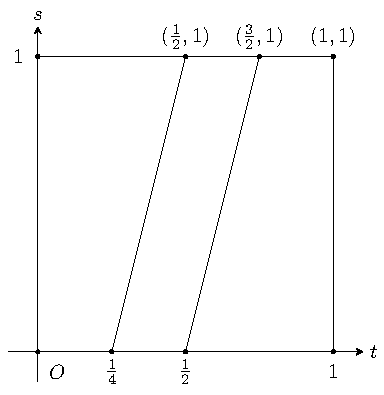
\includegraphics[scale=1]{images/fig_1.pdf}
            \end{center}
            \caption{Dominio de la función $F$.}
        \end{figure}

        para todo $s,t\in I$. Veamos que $F$ es continua... %TODO
    \end{proof}

    Para cualquier punto $x\in X$, denotemos por $\mathscr{I}_x=[i_x]$ a la clase de equivalencia del mapeo identidad, es decir $\cf{i_x}{I}{X}$ es tal que $i_x(t)=x$ para todo $y\in I$. Esta clase tiene la siguiente propiedad fundamental:

    \begin{lema}
        Sea $\mathscr{F}=[f]$ una clase de equivalencia de caminos con punto inicial $x\in X$ y terminal $y\in X$. Entonces, $\mathscr{I}_x\cdot\mathscr{F}=\mathscr{F}$ y $\mathscr{F}\cdot\mathscr{I}_y=\mathscr{F}$.
    \end{lema}

    \begin{proof}
        Solo se probará la primera igualdad, para ello, basta con probar que $i_x\cdot f\sim f$. En efecto, defina la función $\cf{F}{I\times I}{X}$ dada por:
        \begin{equation*}
            F(t,s)=\left\{
                \begin{array}{lcr}
                    x & \textup{ si } & 0\leq t\leq\frac{s}{2}\\
                    f\left(\frac{2t-s}{2-s}\right) & \textup{ si } & \frac{s}{2}\leq t\leq 1\\
                \end{array}
            \right.
        \end{equation*}
        para todo $s,t\in I$. Entonces, $F(t,0)=f(t)$ y $F(t,1)=(e\cdot f)(1)$ siendo $F$ continua. Por tanto, $\mathscr{I}_x\cdot\mathscr{F}=\mathscr{F}$.
    \end{proof}

    En cierto modo, lo que decimos es que la clase $\mathscr{I}_x$ actúa como elemento identidad (\textit{¿De dónde?}).

    \begin{mydef}
        Para cualquier camino $\cf{f}{I}{X}$, $\overline{f}$ denota al camino definido por:
        \begin{equation*}
            \overline{f}(t)=f(1-t),\quad\forall t\in I
        \end{equation*}
        El camino $\overline{f}$ se obtiene recorriendo el camino $f$ en sentido contrario.
    \end{mydef}

    \begin{lema}
        Sea $f$ un camino y denotemos por $\mathscr{F}=[f]$ y $\overline{\mathscr{F}}=[\overline{f}]$, entonces:
        \begin{equation*}
            \mathscr{F}\cdot\overline{\mathscr{F}}=\mathscr{I}_x\quad\textup{y}\quad\overline{\mathscr{F}}\cdot\mathscr{F}=\mathscr{I}_y
        \end{equation*}
        donde $x\in X$ y $y\in X$ son los puntos inicial y terminal de $f$, respectivamnete.
    \end{lema}

    \begin{proof}
        Sólo se probará la primera igualdad, para ello es suficiente con probar que $f\cdot\overline{f}\sim i_x$. Definimos la función $\cf{F}{I\times I}{X}$ por:
        \begin{equation*}
            F(t,s)=\left\{
                \begin{array}{lcr}
                    f(2t) & \textup{ si } & 0\leq t\leq\frac{s}{2}\\
                    f(s) & \textup{ si } & \frac{s}{2}\leq t\leq1-\frac{s}{2}\\
                    f(2-2t) & \textup{ si } & 1-\frac{s}{2}\leq t\leq1\\
                \end{array}
            \right.
        \end{equation*}
        para todo $s,t\in I$. Entonces,
        \begin{equation*}
            \begin{split}
                F(t,0)&=\left\{
                    \begin{array}{lcr}
                        f(2t) & \textup{ si } & 0\leq t\leq0\\
                        f(s) & \textup{ si } & 0\leq t\leq1-0\\
                        f(2-2t) & \textup{ si } & 1-0\leq t\leq1\\
                    \end{array}
                \right.\\
                &=\left\{
                    \begin{array}{lcr}
                        f(0) & \textup{ si } & t=0\\
                        f(0) & \textup{ si } & 0\leq t\leq1\\
                        f(2-2t) & \textup{ si } & t=1\\
                    \end{array}
                \right.\\
                &=\left\{
                    \begin{array}{lcr}
                        x & \textup{ si } & 0\leq t\leq1\\
                        f(0) & \textup{ si } & t=1\\
                    \end{array}
                \right.\\
                &=x\\
            \end{split}
        \end{equation*}
        para todo $t\in I$. Además,
        \begin{equation*}
            \begin{split}
                F(t,1)&=\left\{
                    \begin{array}{lcr}
                        f(2t) & \textup{ si } & 0\leq t\leq\frac{1}{2}\\
                        f(1) & \textup{ si } & \frac{1}{2}\leq t\leq1-\frac{1}{2}\\
                        f(2-2t) & \textup{ si } & 1-\frac{1}{2}\leq t\leq1\\
                    \end{array}
                \right.\\
                &=\left\{
                    \begin{array}{lcr}
                        f(2t) & \textup{ si } & 0\leq t\leq\frac{1}{2}\\
                        f(1-(2t-1)) & \textup{ si } & \frac{1}{2}\leq t\leq1\\
                    \end{array}
                \right.\\
                &=\left\{
                    \begin{array}{lcr}
                        f(2t) & \textup{ si } & 0\leq t\leq\frac{1}{2}\\
                        \overline{f}(2t-1) & \textup{ si } & \frac{1}{2}\leq t\leq1\\
                    \end{array}
                \right.\\
                &=f\cdot\overline{f}(t)\\
            \end{split}
        \end{equation*}
        para todo $t\in I$. La función $F$ es continua... %TODO

        Por tanto, $\mathscr{F}\cdot\overline{\mathscr{F}}$.
    \end{proof}

    En visata de estas propiedades de la clase $\overline{\mathscr{F}}$, de ahora en adelante la denotaremos por $\mathscr{F}^{-1}$.

    Podemos resumir todos los lemas antes probados diciendo que el conjunto de todas las clases de caminos en un espacio $X$ satisfacen los axiomas de grupo, excepto que el producto de dos caminos no siempre está definido. Solventamos este problema con la siguiente definición:

    \begin{mydef}
        Un camino o una clase de camino es llamada \textbf{cerrada} o un \textbf{bucle}, si el punto inicial y terminal son el mimso. El bucle se dice que tiene \textbf{base} en el punto inicial o terminal.
    \end{mydef}

    \begin{theor}
        Sea $X$ un espacio topológico y $x\in X$ un punto fijo. Entonces, el conjunto de todas las clases de caminos cerradas que tienen como punto base a $x$ dotado por la operación $\cdot$, denotado por $\pi(X,x)$ es un grupo llamado \textbf{grupo fundamental} o \textbf{grupo de Poincaré} de $X$ con punto base $x$.
    \end{theor}

    \begin{proof}
        Es un resumen de todos los lemas anteriores.
    \end{proof}

    \begin{obs}
        Para un espacio topológico dado $X$ y $x\in X$, dotamos el grupo fundamental $\pi(X,x)$ de una operación binaria que lo hace de grupo, de ahora en adelante tal operación se denotará al producto de dos clases $[f]$ y $[g]$ por $[f]\cdot[g]$ o por yuxtaposición como $[f][g]=[f\cdot g]$ (no confundir la operación dentro de los paréntesis cuadrados con la composición usual de funciones).

        Si $[f]\in\pi(X,x)$, se denotará a su inverso por $[f]^{-1}$ y, al elemento identidad por $\mathscr{I}$
    \end{obs}

    \begin{propo}
        Sea $X$ un espacio y $x,y\in X$ dos puntos distintos. Si $\cf{\gamma}{I}{X}$ es un camino con punto inicial $x$ y terminal $y$, entonces $\pi(X,x)\cong\pi(X,y)$ (es decir, son grupos isomorfos).
    \end{propo}

    \begin{proof}
        En efecto, defina la función $\cf{u}{\pi(X,x)}{\pi(X,y)}$ dada por:
        \begin{equation*}
            u([f])=[\gamma]^{-1}[f][\gamma]
        \end{equation*}
        Por cursos anteriores de teoría de Grupos, se ve de forma inmediata que esta función es un isomorfismo entre los grupos $\pi(X,x)$ y $\pi(X,y)$.
    \end{proof}

    \begin{cor}
        Sea $X$ un espacio topológico arco-conexo, entonces los grupos $\pi(X,x)$ y $\pi(X,y)$ son isomorfos para todo $x,y\in X$.
    \end{cor}

    La importancia del teorema anterior radica en que el grupo $\pi(X,x)$ tiene propiedades como grupo (es decir, es abeliano, finito, nilpotente, libre, etc...) no debido al punto elegido $x\in X$, sino al espacio mismo $X$, suponiendo que $X$ es arco-conexo.

    En general, no hay un mapeo canónico o isomorfismo natural entre $\pi(X,x)$ y $\pi(X,y)$, ya que a cada elección de camino entre $x$ y $y$ le corresponderá un isomorfismo.

    \section{Efecto de una función continua en el grupo fundamental}

    \begin{obs}
        Para esta sección resultará de utilidad definir el siguiente conjunto, para todo espacio topológico $X$ se define
        \begin{equation*}
            \wp_X = \left\{[f]\Big|\cf{f}{I}{X}\textup{ es una función continua} \right\}
        \end{equation*}
        es decir, estamos tomando todas las clases de caminos de un espacio topológico $X$ (note que no tiene nada que ver con el grupo fundamental, más que con el hecho de que usa las clases de caminos en su definición).
    \end{obs}

    Considere dos espacios topológicos $X$ y $Y$ y sea $\cf{\varphi}{X}{Y}$ una función continua. Si $\cf{f_0,f_1}{I}{X}$ son caminos en $X$, ¿también lo son $\varphi\circ f_0$ y $\varphi\circ f_1$?

    \begin{propo}
        Sean $X$ y $Y$ espacios topológicos, $\cf{f_0,f_1}{I}{X}$ caminos equivalentes. Entonces, $\varphi\circ f_0\sim \varphi\circ f_1$.
    \end{propo}

    \begin{proof}
        Como $f_1\sim f_0$, existe pues una función continua $\cf{F}{I\times I}{X}$ tal que
        \begin{equation*}
            F(x,0)=f_0(x),\quad F(x,1)=f_1(x)
        \end{equation*}
        para todo $x\in I$ y,
        \begin{equation*}
            F(0,t)=f_0(0)=f_1(0),\quad F(1,t)=f_0(1)=f_1(1)
        \end{equation*}
        Considere la función $\cf{G}{I\times I}{Y}$ dada por:
        \begin{equation*}
            G(x,t)=\varphi\circ F(x,t)
        \end{equation*}
        Es claro que esta funciónes continua por ser composición de funciones continuas, además se cumple que
        \begin{equation*}
            \begin{split}
                G(x,0)&=\varphi\circ F(x,0)\\
                &=\varphi (F(x,0))\\
                &=\varphi (f_0(x))\\
                &=\varphi\circ f_0(x)\\
            \end{split}
        \end{equation*}
        para todo $x\in I$. De forma análoga
        \begin{equation*}
            G(x,1)=\varphi\circ f_1(x)
        \end{equation*}
        La otra condición se verifica de forma inmediata, con lo que se concluye que $\varphi\circ f_0\sim \varphi\circ f_1$.
    \end{proof}

    Con la proposición anterior, podemos definir sin problemas una función que mapee clases de caminos en $X$ a clases de caminos en $Y$, a partir de la función continua $\varphi$. Esto se hará con el objetivo de ver qué sucede con el grupo fundamental bajo esta función continua $\varphi_*$.

    \begin{mydef}
        Sean $X$ y $Y$ espacios topológicos y $\cf{\varphi}{X}{Y}$ una función continua. Sea $\cf{f}{I}{X}$ un camino que une a los puntos $x,y\in X$, se define la función $\cf{\varphi_*}{\wp_X}{\wp_Y}$ por
        \begin{equation*}
            \varphi_*([f])=[\varphi\circ f]
        \end{equation*}
        por la proposición anterior, esta función está bien definida.
    \end{mydef}

    Ahora, analizaremos las propiedades de la función $\varphi_*$.
    
    \renewcommand{\theenumi}{\roman{enumi}}

    \begin{propo}
        Sean $X$ y $Y$ espacios topológicos y $\cf{\varphi}{X}{Y}$ una función continua.
        \begin{enumerate}
            \item Si $\cf{f_0,f_1}{I}{X}$ son caminos en $X$ tales que $f_0\cdot f_1$ está definido (por ende, $[f_0]\cdot [f_1]$ lo está), entonces $\varphi_*([f_0]\cdot[f_1])=\varphi_*([f_0])\cdot\varphi_*([f_1])$.
            \item Para cualquier punto $x\in X$, $\varphi_*(\mathscr{I}_x)=\mathscr{I}_{\varphi(x)}$.
            \item Si $\cf{f}{I}{X}$ es un camino, entonces $\varphi_*([f]^{-1})=(\varphi_*([f]))^{-1}$.
        \end{enumerate}
    \end{propo}

    \begin{proof}
        De (i): Veamos primero que el producto $\varphi_*([f_0])\cdot\varphi_*([f_1])$ está bien definido. En efecto, dado a que el producto $[f_0]\cdot [f_1]$ lo está, entonces
        \begin{equation*}
            f_0(1)=f_1(0)
        \end{equation*}
        luego,
        \begin{equation*}
            \varphi\circ f_0(1)=\varphi\circ f_1(0)
        \end{equation*}
        donde $\varphi_*([f_0])=[\varphi\circ f_0]$ y $\varphi_*([f_1])=[\varphi\circ f_1]$, por tanto el producto de ambas clases está definido. Probemos ahora la igualdad. Se tiene que
        \begin{equation*}
            \begin{split}
                \varphi_*([f_0]\cdot[f_1])&=\varphi_*([f_0\cdot f_1])\\
                &=[\varphi\circ (f_0\cdot f_1)]\\
            \end{split}
        \end{equation*}
        siendo
        \begin{equation*}
            f_0\cdot f_1(t)=\left\{
                \begin{array}{lcr}
                    f_0(2t) & \textup{ si } 0\leq t\leq \frac{1}{2}\\
                    f_1(2t-1) & \textup{ si } \frac{1}{2}\leq t\leq 1\\
                \end{array}
            \right.,\quad\forall t\in I
        \end{equation*}
        por ende,
        \begin{equation*}
            \begin{split}
                \varphi\circ (f_0\cdot f_1)(t)&=\left\{
                    \begin{array}{lcr}
                        \varphi(f_0(2t)) & \textup{ si } 0\leq t\leq \frac{1}{2}\\
                        \varphi(f_1(2t-1)) & \textup{ si } \frac{1}{2}\leq t\leq 1\\
                    \end{array}
                \right.\\
                &=\left\{
                    \begin{array}{lcr}
                        \varphi\circ f_0(2t) & \textup{ si } 0\leq t\leq \frac{1}{2}\\
                        \varphi\circ f_1(2t-1) & \textup{ si } \frac{1}{2}\leq t\leq 1\\
                    \end{array}
                \right.\\
                &=(\varphi\circ f_0)\cdot (\varphi\circ f_1)(t),\quad\forall t\in I\\
            \end{split}
        \end{equation*}
        luego entonces
        \begin{equation*}
            \begin{split}
                [\varphi\circ (f_0\cdot f_1)]&=[(\varphi\circ f_0)\cdot (\varphi\circ f_1)]\\
                &=[\varphi\circ f_0]\cdot [\varphi\circ f_1]\\
                &=\varphi_*([f_0])\cdot \varphi_*([f_1])\\
            \end{split}
        \end{equation*}
        lo que prueba el resultado.

        De (ii) y (iii): Ejercicio.
    \end{proof}

    Por estas razones, llamaremos a $\varphi_*$ un \textit{homomorfismo} u \textit{homomorfismo inducido por $\varphi$}.

    \begin{propo}
        En el contexto de la proposición anterior, si $Z$ es un espacio topológico y $\cf{\psi}{Y}{Z}$ es una función continua, entonces
        \begin{equation*}
            (\psi\circ\varphi)_*=\psi_*\circ\varphi_*
        \end{equation*}
    \end{propo}

    \begin{proof}
        Es claro que la composición de ambas funciones está bien definida. Probaremos ahora la igualdad, sea $\cf{f}{I}{X}$ un camino, entonces:
        \begin{equation*}
            \begin{split}
                (\psi\circ\varphi)_*([f])&=[\psi\circ\varphi\circ f]\\
                &=[\psi\circ(\varphi\circ f)]\\
                &=\psi_*([\varphi\circ f])\\
                &=\psi_*(\varphi_*([f]))\\
                &=\psi_*\circ \varphi_*([f])\\
            \end{split}
        \end{equation*}
        lo que prueba la igualdad.
    \end{proof}

    \begin{excer}
        Sea $X$ espacio topológico y $\cf{i}{X}{X}$ la función identidad, entonces
        \begin{equation*}
            i_*([f])=[f]
        \end{equation*}
        para todo camino $\cf{f}{I}{X}$ en $X$.
    \end{excer}

    \begin{proof}
        Ejercicio.
    \end{proof}

    \begin{obs}
        En otras palabras, lo que nos dice la proposición anterior es que el mapeo $i_*$ reestringido a $\pi(X,x)$ coincide con la identidad de $\bbm{1}_{\pi(X,x)}$, y que
        \begin{equation*}
            i_*=\bbm{1}_{\wp_X}
        \end{equation*}
    \end{obs}
    
    \begin{cor}
        Sean $X$ y $Y$ espacios topológicos y $\cf{\varphi}{X}{Y}$ una función continua y $x\in X$. La función $\varphi_*$ restringida a $\pi(X,x)\subseteq\wp_X$ es un homomorfismo entre $\pi(X,x)$ y $\pi(Y,\varphi(x))$. Más aún, si $\varphi$ es homeomorfismo, entonces $\varphi_*$ reestringida a $\pi(X,x)$ es isomorfismo.
    \end{cor}

    \begin{proof}
        El hecho de que sea homomorfismo es inmediato de la proposición anterior y de que si $f$ es un bucle con base en $x$, entonces
        \begin{equation*}
            \varphi_*([f])=[\varphi\circ f]
        \end{equation*}
        es la clase del camino $\varphi\circ f$, el cual es un bucle con base en $\varphi(x)$.

        Veamos ue si $\varphi$ es homeomorfismo entonces $\varphi_*$ es isomorfismo. En efecto, como es homeomorfismo existe una función $\cf{\varphi^{-1}}{Y}{X}$ continua que es la inversa de $\varphi$.

        Se sigue de la proposición anterior que
        \begin{equation*}
            (\bbm{1}_X)_*=(\varphi\circ\varphi^{-1})_*=\varphi_*\circ\varphi_*^{-1}
        \end{equation*}
        donde $\bbm{1}_X$ es la identidad de $X$, luego
        \begin{equation*}
            \varphi_*\circ\varphi_*^{-1}=\bbm{1}_{\wp_X}
        \end{equation*}
        de forma análoga se sigue que
        \begin{equation*}
            \varphi_*^{-1}\circ\varphi_*=\bbm{1}_{\wp_Y}
        \end{equation*}
        por tanto, la función $\varphi_*$ es invertible, luego $\varphi_*$ reestringida a $\pi(X,x)$ es invertible, con inversa la reestricción de $\varphi_*^{-1}$ a $\pi(Y,\varphi(x))$. Así, $\varphi_*$ es isomorfismo.
    \end{proof}

    \section{Nociones geométricas subyacentes}

    Para continuar con el estudio de la función inducida $\varphi_*$, es necesario introducir algunos conceptos geométricos relevantes,

    \begin{mydef}
        Sean $X$ y $Y$ espacios topológicos. Dos funciones continuas $\cf{\varphi_0,\varphi_1}{X}{Y}$ son \textbf{homotópicas} si existe una función continua $\cf{\Phi}{X\times I}{Y}$ tal que para todo $x\in X$:
        \begin{equation*}
            \Phi(x,0)=\varphi_0(x)\quad\textup{y}\quad\Phi(x,1)=\varphi_1(x)
        \end{equation*}
        además, para denotar que son homotópicas, se usará el símbolo $\varphi_0\simeq\varphi_1$.
    \end{mydef}

    \begin{obs}
        En ciertos casos, será más conveniente denotar a la homotopía como la familia de funciones $\left\{\varphi_t \right\}_{ t\in I}$ tal que cada una es continua y que el mapeo $t\mapsto \varphi_t$ es continuo en el espacio de funciones continuas, donde
        \begin{equation*}
            \Phi(x,t)=\varphi_t(x),\quad\forall x\in X,\forall t\in I
        \end{equation*}
        y por esta razón, se denotará por $\varphi_t$ a $\Phi$.
    \end{obs}

    \begin{propo}
        Sean $X$ y $Y$ espacios topológicos. Considere el conjunto:
        \begin{equation*}
            \mathcal{F}=\left\{\cf{\varphi}{X}{Y}\Big|f\textup{ es una función continua} \right\}
        \end{equation*}
        entonces, $\simeq$ es una relación de equivalencia sobre $\mathcal{F}$.
    \end{propo}

    \begin{proof}
        Ejercicio.
    \end{proof}

    \begin{obs}
        Para aquellos que han tomado algún curso en teoría de categorías, verán de forma casi inmediata que esta relación de equivalencia induce una partición en la clase de todos los morfismos entre espacios topológicos.
    \end{obs}

    La idea detrás de la homotopía es intentar deformar de forma continua una función en la otra, conservando la continuidad de las funciones, veamos que si
    \begin{equation*}
        \varphi_t(x)=\Phi(x,t)
    \end{equation*}
    para todo $x\in X$ y todo $t\in I$, entonces la función $\cf{\varphi_t}{X}{Y}$ es continua.

    Por esta razón es que comúnmente se habla de homotopía como la deformación continua de una función.

    \begin{obs}
        En otros contextos, resulta más familiar decir que dos funciones son homotópicas si pueden ser unidas con un arco en el espacio de todas las funciones continuas que van de $X$ en $Y$.
    \end{obs}

    \begin{mydef}
        Dos funciones $\cf{\varphi_0,\varphi_1}{X}{Y}$ entre los espacios topológicos $X$ y $Y$ son \textbf{homotópicas relativas al subconjunto $A$ de $X$} si existe una función continua $\cf{\Phi}{X\times I}{Y}$ tal que
        \begin{equation*}
            \begin{split}
                \varphi(x,0)=\varphi_0(x) & \quad\forall x\in X\\
                \varphi(x,1)=\varphi_1(x) & \quad\forall x\in X\\
                \varphi(a,t)=\varphi_0(a)=\varphi_1(a) & \quad\forall a\in A\textup{ y }\forall t\in I \\
            \end{split}
        \end{equation*}
    \end{mydef}

    Básicamente la deformación continua es tal que deja al subconjunto $A$ sin modificarse en el proceso de deformación.

    \begin{theor}
        Sean $\cf{\varphi_0,\varphi_1}{X}{Y}$ funciones entre dos espacios topológicos y $x\in X$. Suponga que son homotópicas $\varphi_0$ y $\varphi_1$ relativas al conjunto $\left\{u \right\}$, entonces
        \begin{equation*}
            \cf{{\varphi_0}_*={\varphi_1}_*}{\pi(X,u)}{\pi(Y,\varphi_0(u))}
        \end{equation*}
        esto es, los homomorfismos inducidos son el mismo.
    \end{theor}

    \begin{proof}
        Sea $\cf{f}{I}{X}$ un bucle que une a $x$ consigo mismo. Como $\varphi_0$ y $\varphi_1$ son homotópicas relativas al conjunto $\left\{u\right\}$, entonces existe una función continua $\cf{\Phi}{X\times I}{Y}$ tal que
        \begin{equation*}
            \begin{split}
                \Phi(x,0)=\varphi_0(x) & \quad\forall x\in X\\
                \Phi(x,1)=\varphi_1(x) & \quad\forall x\in X\\
                \Phi(u,t)=\varphi_0(u)=\varphi_1(u) & \quad\forall t\in I
            \end{split}
        \end{equation*}
        por tanto, se tiene para el camino $f$ que la función $\cf{G}{I\times I}{Y}$ dada por
        \begin{equation*}
            G(s,t)=\Phi(f(s),t),\quad\forall s,t\in I
        \end{equation*}
        es continua, y cumple que
        \begin{equation*}
            F(s,0)=\varphi_0\circ f(s)\quad\textup{ y }F(s,1)=\varphi_1\circ f(s)
        \end{equation*}
        para todo $s\in I$. Además,
        \begin{equation*}
            \begin{split}
                F(0,t)&=\Phi(f(0),t)=\Phi(u,t)=\varphi_0(u)=\varphi_1(u)\\
                F(1,t)&=\Phi(f(1),t)=\Phi(u,t)=\varphi_0(u)=\varphi_1(u)\\
            \end{split}
        \end{equation*}
        para todo $t\in I$. Por tanto, los caminos
        \begin{equation*}
            \varphi_0\circ f\quad\textup{ y }\varphi_1\circ f
        \end{equation*}
        son equivalentes, luego:
        \begin{equation*}
            \begin{split}
                {\varphi_0}_*([f])&=[\varphi_0\circ f]\\
                &=[\varphi_1\circ f]\\
                &={\varphi_1}_*([f])\\
            \end{split}
        \end{equation*}
        dado a que el bucle $f$ fue arbitrario, se sigue que
        \begin{equation*}
            {\varphi_0}_*={\varphi_1}_*
        \end{equation*}
    \end{proof}

    Ahora nos dedicaremos a aplicar estos resultados.

    \begin{mydef}
        Un subconjunto $A\subseteq X$ de un espacio topológico es un \textbf{repliegue} de $X$ si existe una función continua $\cf{r}{X}{A}$ (llamada \textbf{retración}) tal que $r(a)=a$ para todo $a\in A$.
    \end{mydef}

    La condición de la definición antes mencionada, es una condición muy fuerte, ya que no todo espacio la cumple para cualquier conjunto $A$ arbitrario. Vea estos dos ejemplos:

    \begin{exa}
        Considere $X=\mathbb{R}^2\backslash\left\{(0,0)\right\}$ y tomemos $A=\mathbb{R}+(1,0)$. ¿Existe un repliegue de $X$ en $A$?
    \end{exa}

    \begin{exa}
        Considere el espacio $X$ como la cinta de Möbius y sea $A$ el círculo central de la cinta. ¿Es $A$ una retracción de $X$? En caso de que sea ¿cuál es una posible retracción?
    \end{exa}

    Sea ahora $\cf{r}{X}{A}$ una retración e $\cf{i}{A}{X}$ el mapeo inclusión. Para cualquier punto $a\in A$ se consideran los homomorfismos inducidos:
    \begin{equation*}
        \begin{split}
            \cf{i_*}{\pi(A,a)}{\pi(X,a)}\\
            \cf{r_*}{\pi(X,a)}{\pi(A,a)}\\
        \end{split}
    \end{equation*}
    siendo éstos tales que $r\circ i=\bbm{1}_{A}$, debe suceder entonces que $r_*\circ i_*=\bbm{1}_{\pi(A,a)}$ es el homomorfismo identidad.
    
    Se sigue entonces que
    \begin{itemize}
        \item $i_*$ es monomorfismo.
        \item $r_*$ es epimorfismo.
    \end{itemize}

    Estos resultados se usarán más adelante para probar que ciertos subespacios no son repliegues del espacio original.

    \begin{mydef}
        Un subconjunto $A$ de $X$ es un \textbf{repliegue de deformación} de $X$ si existe una retracción $\cf{r}{X}{A}$ y una homotopía $\cf{F}{X\times I}{X}$ tal que
        \begin{equation*}
            \begin{split}
                \left.
                \begin{array}{rcl}
                    F(x,0) & = & x\\
                    F(x,1) & = & r(x)\\
                \end{array}
            \right\}, & \quad\forall x\in X\\
            F(a,t)=a,\quad&\forall a\in A, \forall t\in I\\
            \end{split}
        \end{equation*}
    \end{mydef}

    En otras palabras, la definición anterior es equivalente a decir que $r\simeq \bbm{1}_X$ y es tal que $F(A\times I)=A$.
    
    \begin{theor}
        Si $A$ es un repliegue de deformación de $X$, entonces el mapeo inclusión $\cf{i}{A}{X}$ induce un isomorfismo entre $\pi(A,a)$ y $\pi(X,a)$ para todo $a\in A$.
    \end{theor}

    \begin{proof}
        Sea $a\in A$. Ya se sabe de la parte anterior que $i_*$ es un monomorfismo. Para probar que es isomorfismo, basta con probar que
        \begin{equation*}
            \cf{i_*\circ r_*}{\pi(X,a)}{\pi(X,a)}
        \end{equation*}
        coincide con $\bbm{1}_{\pi(X,a)}$. Afirmamos que $i\circ r$ es homotópico a $\bbm{1}_X$ respecto a $\left\{a\right\}$. En efecto, como $A$ es repliegue de deformación de $X$, entonces existe una homotopía $\cf{F}{X\times I}{Y}$ tal que
        \begin{equation*}
            \begin{split}
                \left.
                \begin{array}{rcl}
                    F(x,0) & = & \bbm{1}_X(x)\\
                    F(x,1) & = & r(x)\\
                \end{array}
            \right\} & \quad\forall x\in X\\
            F(a',t)=a',\quad&\forall a'\in A, \forall t\in I\\
            \end{split}
        \end{equation*}
        y, como $i\circ r(x)=x$, para todo $x\in X$ (por ser $i$ el mapeo inclusión), se sigue que
        \begin{equation*}
            \begin{split}
                \left.
                \begin{array}{rcl}
                    F(x,0) & = & \bbm{1}_X(x)\\
                    F(x,1) & = & i\circ r(x)\\
                \end{array}
            \right\} & \quad\forall x\in X\\
            F(a,t)=a,\quad&\forall t\in I\\
            \end{split}
        \end{equation*}
        lo cual prueba la afirmación. Se sigue del teorema anterior que
        \begin{equation*}
            i_*\circ r_*=(i\circ r)_*=\bbm{1}_{\pi(X,a)}
        \end{equation*}
    \end{proof}

    Este teorema que acabamos de probar nos va a servir de dos cosas:
    \begin{itemize}
        \item Se usará para probar que dos espacios tienen grupos fundamentales isomorfos.
        \item Un subespacio $A$ no es un repliegue de deformación de $X$ si los grupos fundamentales no son isomorfos.
    \end{itemize}

    En particular se usará el segundo punto para probar que ciertos repliegues no son repliegues de deforamción.

    \begin{mydef}
        Un espacio topológico $X$ es \textbf{contraíble a un punto} si existe $x_0\in X$ tal que $\left\{x_0\right\}$ es un repliegue de deformación de $X$.
    \end{mydef}

    \begin{propo}
        Si $X$ es un espacio contraíble a un punto, entonces es arco-conexo.
    \end{propo}

    \begin{proof}
        Sea $x_0\in X$ tal que $X$ es repliegue de deformación de $X$, entonces existe una homotopía tal que:
        \begin{equation*}
            \left.
                \begin{split}
                    F(x,0) & = x \\
                    F(x,1) & = x_0 \\
                \end{split}
            \right\},\quad\forall x\in X
        \end{equation*}
        y,
        \begin{equation*}
            F(x_0,t)=x_0,\quad\forall t\in I
        \end{equation*}
        Para cada $x\in X$ defina $\cf{f_x}{I}{X}$ dada por:
        \begin{equation*}
            f_x(t)=F(x,t)
        \end{equation*}
        entonces, $f_x$ es una función continua tal que
        \begin{equation*}
            f_x(0)=F(x,0)=x\quad\textup{y}\quad f_x(1)=F(x,1)=x_0
        \end{equation*}
        por tanto, para cada $x\in X$ existe un arco que une a $x_0$ con $x$, luego $X$ es arco-conexo.
    \end{proof}

    \begin{mydef}
        Un espacio topológico es \textbf{simplemente conexo} si es arco-conexo y $\pi(X,x)=\langle e\rangle$ para algún (y por ende para cualquier) $x\in X$.
    \end{mydef}

    \begin{cor}
        Si un espacio es contraíble a un punto, entonces es simplemente conexo.
    \end{cor}

    \begin{proof}
        Es inmediato del hecho que el grupo fundamental del espacio topológico consistente de un solo elemento es tal que su grupo fundamental es trivial y de la proposición anterior.
    \end{proof}

    \section{Simplificación de algunos grupos fundamentales}

    \begin{mydef}
        Un subconjunto $X$ del espacio $\mathbb{R}^n$ es llamado \textbf{convexo} si la línea uniendo cualesquiera dos puntos de $X$ está contenida en $X$.
    \end{mydef}

    Afirmamos que todo subconjunto convexo $X$ de $\mathbb{R}^n$ es contraíble a un punto. En efecto, sea $x_0\in X$ arbitrario fijo. Considere la función $\cf{f}{X\times I}{X}$ dada por:
    \begin{equation*}
        F(x,t)=(1-t)x+tx_0
    \end{equation*}

    \begin{exa}
        Todo subconjunto convexo de $\mathbb{R}^n$ es contraíble a un punto.
    \end{exa}

    \begin{proof}
        Sea $X$ un subconjunto convexo de $\mathbb{R}^n$ y $x_0\in X$. Primero debemos dar una retracción de $X$ en $\left\{ x_0\right\}$. Sea
        \begin{equation*}
            r(x)=x_0\quad\forall x\in X
        \end{equation*}
        es claro que esta función es continua. Para ver que $X$ es contraíble a $\left\{x_0\right\}$ veamos que la función $\cf{F}{X\times I}{X}$ dada por:
        \begin{equation*}
            F(x,t)=(1-t)x+tx_0\quad\forall x\in X,t\in I
        \end{equation*}
        (esta función es es básicamente para $x\in X$ fijo el segmento que une a $x$ con $x_0$, y al variar $x$ se pasan por todos los posibles segmentos que unen con $x_0$). Esta función es continua y efectivamente tiene como contradiminio $X$, ya que el espacio $X$ es convexo. Además:
        \begin{equation*}
            \begin{split}
                \left.
                    \begin{array}{rcl}
                        F(x,0) & = & x \\
                        F(x,1) & = & x_0 = r(x) \\
                    \end{array}
                \right\},\quad&\forall x\in X\\
                F(x_0,t)=x_0,\quad&\forall t\in I\\
            \end{split}
        \end{equation*}
        por tanto, $\left\{x_0\right\}$ es repliegue de deformación de $X$, i.e. $X$ es contraíble a un punto.
    \end{proof}

    \begin{mydef}
        Un subconjunto no vacío $X$ de $\mathbb{R}^n$ se dice que tiene \textbf{forma de estrella respecto a $x_0\in X$} si el segmento que une a $x_0$ con $x$ está contenido en $X$, para todo $x\in X$.
    \end{mydef}    

    Como en el ejemplo anterior, se prueba de forma análoga que cualquier conjunto con forma de estrella es contraíble a un punto.

    \begin{propo}
        Sea $X\subseteq\mathbb{R}^n$ un subconjunto con forma de estrella respecto a algún $x\in X$. Entonces $X$ es contraíble a un punto y por ende, simplemente conexo.
    \end{propo}

    \begin{proof}
        Ejercicio.
    \end{proof}

    \begin{exa}
        Afirmamos que la $(n-1)$-esfera unitaria $\mathbb{S}^{ n-1}$
        \begin{equation*}
            \mathbb{S}^{ n-1}=\left\{x\in\mathbb{R}^n\Big|\|x\|=s1 \right\}
        \end{equation*}
        es una deformación de repliegue de $\mathbb{R}^n-\left\{0\right\}$ para todo $n\in\mathbb{N}$.
    \end{exa}

    \begin{proof}
        En efecto, sea $n\in\mathbb{N}$ y considere el repliegue $\cf{r}{\mathbb{R}^n-\left\{0\right\}}{\mathbb{S}^{ n-1}}$ dado por
        \begin{equation*}
            r(x)=\frac{x}{\|x\|},\quad\forall x\in\mathbb{R}^n-\left\{0\right\}
        \end{equation*}
        Claramente esta es una función continua. Construímos la homotopía $\cf{F}{(\mathbb{R}^n-\left\{0\right\})\times I}{\mathbb{R}^n-\left\{0\right\}}$ dada por:
        \begin{equation*}
            F(x,t)=(1-t)x+t\cdot\frac{x}{\|x\|},\quad\forall x\in \mathbb{R}^n-\left\{0\right\}, \forall t\in I
        \end{equation*}
        Es claro que esta función es continua, para la que se cumple    que
        \begin{equation*}
            \begin{split}
                \left.
                    \begin{array}{rcl}
                        F(x,0) & = & x\\
                        F(x,0) & = & r(x)\\
                    \end{array}
                \right\},&\quad\forall x\in\mathbb{R}^n-\left\{0\right\}\\
            \end{split}
        \end{equation*}
        y,
        \begin{equation*}
            \begin{split}
                F(s,t)&=(1-t)s+t\cdot\frac{s}{\|s\|}\\
                &=(1-t)s+ts\\
                &=s,\quad\forall s\in\mathbb{S}^{ n-1},\quad\forall t\in I \\
            \end{split}
        \end{equation*}
        Por tanto, $\mathbb{S}^{ n-1}$ es una deformación de retracción de $\mathbb{R}^n-\left\{0\right\}$.
    \end{proof}
    \begin{propo}
        Un espacio $X$ es simplemente conexo si y sólo si todos los caminos que conecten cualesquier dos par de puntos en $X$ son equivalentes, esto es, que para cualquier par de puntos solo hay una clase de caminos.
    \end{propo}

    \begin{proof}
        $\Rightarrow$): Suponga que $X$ es simplemente conexo, entonces es arco-conexo y $\pi(X,x)=\langle e\rangle$. Sean $\cf{f,g}{I}{X}$ un camino con puntos extremos $y$ y $z$ inicial y terminal, respectivamente. Entonces $f\cdot\overline{g}$ es un bucle con punto base $y$, luego:
        \begin{equation*}
            \begin{split}
                [f]&=[f]\cdot[i_z]\\
                &=[f]\cdot[\overline{g}\cdot g]\\
                &=[f\cdot\overline{g}]\cdot[g]\\
                &=[i_y]\cdot[g]\\
                &=[g]\\
            \end{split}
        \end{equation*}
        pues, $[\overline{g}\cdot g]\in\pi(X,z)=\langle e\rangle$ y $[f\cdot\overline{g}]\in\pi(X,z)=\langle e\rangle$. Luego, $f\sim g$.

        $\Leftarrow)$: Es inmediata. %TODO
    \end{proof}

    \section{Espacios Recubridores}

    \subsection{Preeliminares}

    Para determinar el grupo fundamental del círculo, será necesario introducir teoría sobre espacios recubridores.
    
    \begin{mydef}
        Sea $(X,\tau)$ un espacio topológico. Un \textbf{espacio recubridor} o \textbf{cubridor} de $X$ consiste de una tupla $(\widetilde{X},p)$ siendo $\widetilde{X}$ un espacio topológico y $\cf{p}{\widetilde{X}}{X}$ una función tal que
        \begin{itemize}
            \item Para cada punto $x\in X$ existe una vecindad arco-conexa $U$ tal que cada componente arco-conexa de $p^{-1}(U)$ es homeomorfa a $U$ bajo la reestricción de $p$ a la componente.
        \end{itemize}
        Cada abierto $U$ que satisfaga la condición anterior es llamado \textbf{vecindad elemental} y se dice que $U$ es \textbf{recubierto uniformemente}. La funcón $\cf{p}{\widetilde{X}}{X}$ es llamada habitualmente \textbf{proyección}.
    \end{mydef}

    Veamos algunos ejemplos para clarificar mejor las ideas.

    \begin{exa}
        Si $X$ es un espacio topológico y $\cf{\bbm{1}_X}{X}{X}$ denota a la función identidad, entonces $(X,\bbm{1}_X)$ es un espacio recubridor de $X$.
        
        Similarmente, si $X,Y$ son espacios topológicos y $\cf{f}{X}{Y}$ es un homeomorfismo, entonces $(X,f)$ es un espacio recubridor de $Y$.
    \end{exa}

    \begin{exa}
        Si $(\widetilde{X},p)$ y $(\widetilde{Y},q)$ son espacios recubridores de $X$ y $Y$, respectivamente entonces, $(\widetilde{X}\times\widetilde{Y},p\times q)$ es un espacio recubridor de $X\times Y$, donde
        \begin{equation*}
            p\times q(x,y)=(p(x),q(y)),\quad\forall (x,y)\in X\times Y
        \end{equation*}
    \end{exa}

    \begin{proof}
        Ejercicio.
    \end{proof}

    \begin{exa}
        Considere la función $\cf{p}{\mathbb{R}}{\mathbb{S}^1}$ dada por:
        \begin{equation*}
            p(s)=(\cos 2\pi s,\sin 2\pi s),\quad\forall s\in I
        \end{equation*}
        (donde $\mathbb{R}$ está dotado de la topología usual). Entonces $(\mathbb{R},p)$ es un espacio recubridor de $\mathbb{S}^1$. Cualquier subintervalo abierto del círculo sirve como vecindad elemental. Este ejemplo deberá ser tomado en cuenta ya que será de utilidad más adelante.
    \end{exa}

    \begin{propo}
        La función $\cf{p}{\mathbb{R}}{\mathbb{S}^1}$ definida anteriormente hace de la tupla $(\mathbb{R},p)$ un espacio recubridor de $\mathbb{S}^1$. Más aún, todo arco abierto en $\mathbb{S}^1$ es recubierto uniformemente.
    \end{propo}

    \begin{proof}
        Para la primera parte, sea $x=(\cos2\pi s,\sin2\pi s)\in\mathbb{S}^1$ (con $s\in[0,1[$). La función $p$ es continua, por lo que el abierto
        \begin{equation*}
            U=\left\{(\cos2\pi(s+r),\sin2\pi (s+r))\Big|r\in[0,1/4[ \right\}
        \end{equation*}
        en $\mathbb{S}^1$ es tal que $p^{-1}(U)$ es abierto. Es claro que
        \begin{equation*}
            p^{-1}(U)=\bigcup_{ s\in\mathbb{Z}}]s-1/4,s+1/4[
        \end{equation*}
        siendo cada uno de los intervalos disjuntos en la unión homeomorfo a $U$.

        Notemos que podemos cambiar $U$ por un arco abierto y el resultado sigue siendo válido. 
    \end{proof}

    Usando uno de los ejemplos anteriores, uno puede construir dos espacios recubridores del toro (recuerde que $\mathbb{T}=\mathbb{S}^1\times\mathbb{S}^1$), a saber:

    \begin{equation*}
        \cf{p}{\mathbb{R}^2}{\mathbb{T}=\mathbb{S}^1\times\mathbb{S}^1}\quad\textup{y}\quad\cf{q}{\mathbb{R}\times\mathbb{S}^1}{\mathbb{T}=\mathbb{S}^1\times\mathbb{S}^1}
    \end{equation*}
    (donde las funciones son fácilmente construíbles a partir de los ejemplos anteriores).

    \begin{obs}
        Para más ejemplos desarrollados explícitamente, se recomienda checar: \textit{A basic course in Algebraic Topology} de Massey W. S.

        Más adelante se abordarán estos ejemplos, el objetivo actual no tiene mucho que ver con el análisis de los mismos, sino con la prueba de un resultado imprescindible.
    \end{obs}

    \begin{mydef}
        Una función continua $\cf{f}{X}{Y}$ es un \textbf{homeomorfismo local}, si para cada punto $x\in X$ existe una vecindad abierta $V$ de $x$ tal que $f(V)$ es abierto y $f\big|_{V}$ es un homeomorfismo.
    \end{mydef}

    \begin{obs}
        De la definición de espacio recubridor se verifica fácilmente que $p$ es un homeomorfismo local.
    \end{obs}

    \begin{exa}
        Si $(\widetilde{X},p)$ es un espacio recubridor de $X$ y $V$ es un subconjunto propio de $\widetilde{X}$ conexo y abierto, entonces $p\big|_{V}$ es un homeomorfismo local, pero $(V,p\big|_{V})$ no es un espacio recubridor de $X$.
    \end{exa}

    \begin{proof}
        Observe que puede suceder que $p\big|_{V}$ no sea suprayectiva
    \end{proof}

    \begin{propo}
        Todo homomorfismo local es una función abierta.
    \end{propo}

    \begin{proof}
        Sea $\cf{f}{X}{Y}$ un homomorfismo local y $U\subseteq X$ abierto no vacío, debemos probar que $f(U)$ es abierto.

        Sea $x\in U$, como $f$ es homomorfismo local, existe un abierto $V_x\subseteq X$ tal que $f\big|_{ V_x}$ es homomorfismo. En particular se tiene que $U\cap V_x$ es un abierto en $X$ contenido en $V_x$, por ser homomorfismo, se sigue que
        \begin{equation*}
            f|_{V_x}(U\cap V_x)
        \end{equation*}
        es abierto en $Y$, pero
        \begin{equation*}
            f(U)=f\left(\bigcup_{ x\in U} U\cap V_x\right)=\bigcup_{ x\in U} f(U\cap V_x)=\bigcup_{ x\in U} f\big|_{ V_x}(U\cap V_x)
        \end{equation*}
        donde todos los conjuntos en la unión de la derecha son abiertos, luego $f(U)$ es abierto.

        Se sigue al ser $U$ arbitrario que $f$ es abierta.
    \end{proof}

    \begin{cor}
        Si $(\widetilde{X},p)$ es un espacio recubridor de $X$, entonces $p$ es una función abierta.
    \end{cor}

    \begin{proof}
        Inmediata del teorema anterior.
    \end{proof}

    \subsection{Levantamiento de caminos en un espacio recubridor}

    En esta parte se pretende probar algunos lemas que resultarán relevantes para algunos resultados que se verán posteriormente, relacionados con los espacios recubridores (y sobre todo con la determinación de grupos fundamentales).

    Antes, se probarán algunos resultados sobre espacios métricos.

    \begin{mydef}
        Sea $(X,d)$ un espacio métrico y $A\subseteq X$ un conjunto no vacío. Para cada $x\in X$ definimos la \textbf{distancia de $x$ a $A$}, como
        \begin{equation*}
            d(x,A)=\inf\left\{d(x,a)\Big|a\in A \right\}
        \end{equation*}
    \end{mydef}

    En Análisis Matemático I se probó que esta función como una función de $X$ en $\mathbb{R}^+\cup\left\{0\right\}$ es continua, para la que se cumple que
    \begin{equation*}
        d(x,A)-d(y,A)\leq d(x,y),\quad\forall x,y\in X
    \end{equation*}

    \begin{mydef}
        Sea $(X,d)$ un espacio métrico y $A\subseteq X$ un conjunto acotado no vacío. El \textbf{diámetro de $A$} es el número real:
        \begin{equation*}
            D(A)=\sup\left\{d(a_1,a_2)\Big|a_1,a_2\in A \right\}
        \end{equation*}
    \end{mydef}

    \begin{lema}[\textbf{Lema del número de Lebesgue}]
        Sea $(X,d)$ un espcio métrico y $\mathcal{A}=\left\{A_i \right\}_{ i\in I}$ una cubierta abierta de $(X,d)$. Si $X$ es compacto, entonces existe $\delta>0$ tal que para cada subconjunto de $X$ con diámetro menor que $\delta$ existe $i_0\in I$ tal que $A_{ i_0}$ lo contiene. 

        $\delta$ es llamado el \textbf{número de Lebesgue de $\mathcal{A}$}.
    \end{lema}

    \begin{proof}
        Se tienen dos casos:
        \begin{itemize}
            \item Si $X$ está totalmente contenido en algún $A_i$, tomando $\delta=1$ se tiene el resultado.
            \item Suponga que $X$ no está totalmente contenido en algún $A_i$. COomo $X$ es compacto, existen $A_{ i_1},...,A_{ i_n}$ tales que
            \begin{equation*}
                X=\bigcup_{ j=1}^n A_{ i_j}
            \end{equation*}
            Para cada $j\in\natint{1,n}$, sea
            \begin{equation*}
                C_j=X-A_{ i_j}
            \end{equation*}
            defina la función $\cf{f}{X}{\mathbb{R}}$ dada por:
            \begin{equation*}
                f(x)=\frac{1}{n}\sum_{ j=1}^n d(x,C_j)
            \end{equation*}
            (esta distancia es la media de las distancias a cualquier conjunto $C_j$). Probaremos que $f(x)>0$ para todo $x\in X$. Sea $x\in X$, entonces existe $j_0\in\natint{1,n}$ tal que $x\in A_{ i_{ j_0}}$, como $A_{ i_{ j_0}}$ es abierto, existe $\varepsilon>0$ tal que
            \begin{equation*}
                B_d(x,\varepsilon)\subseteq A_{ i_{ j_0}}
            \end{equation*}
            Entonces, $f(x)\geq\frac{\varepsilon}{n}>0$. Como $f$ es una función continua (por ser suma de funciones continuas) en un compacto, alcanza su máximo y su mínimo, en particular alcanza su mínimo, digamos $\delta>0$ (tiene que ser positivo ya que en caso contrario no se cumpliría la desigualdad enunciada anteriormente).

            Afirmamos que $\delta>0$ es el número de Lebesgue. Sea $B\subseteq X$ no vacío tal que $D(B)<\delta$, sea $x_0\in B$, entonces
            \begin{equation*}
                B\subseteq B_d(x,\delta)
            \end{equation*}
            y, además
            \begin{equation*}
                \delta\leq f(x_0)\leq d(x_0,C_m)=d(x_0,X-A_{ i_m})
            \end{equation*}
            siendo $m\in\natint{1,n}$ tal que $d(x_0,C_m)$ es el máximo de las distancias a cualquier $C_j$. Luego $x_0\in A_{ i_m}$. Se sigue entonces que
            \begin{equation*}
                B\subseteq A_{ i_m}
            \end{equation*}
        \end{itemize}
        por los incisos anteriores se tiene el resultado.
    \end{proof}

    \begin{lema}
        Sea $(\widetilde{X},p)$ un espacio recubridor de $X$ y sea $Y$ un espacio conexo. Dadas dos funciones $\cf{f_0,f_1}{Y}{\widetilde{X}}$ continuas tales que
        \begin{equation*}
            p\circ f_0=p\circ f_1
        \end{equation*}
        se tiene que el conjunto
        \begin{equation*}
            F=\left\{y\in Y\Big|f_0(y)=f_1(y) \right\}
        \end{equation*}
        es vacío o es todo $Y$.
    \end{lema}

    \begin{proof}
        Como $Y$ es conexo, basta con probar que el conjunto $F$ es abierto y cerrado. Sin pérdida de generalidad podemos asumir que $F$ es no vacío.
        \begin{itemize}
            \item \textit{$F$ es cerrado}: Sea $y\in\overline{F}$ y tomemos
            \begin{equation*}
                x=p\circ f_0(y)=p\circ f_1(y)
            \end{equation*}
            Sea $U$ una vecindad elemental de $x$ y sean $V_0$ y $V_1$ las componentes arco-conexas de $p^{-1}(U)$ que contienen a $f_0(y)$ y $f_1(y)$, respectivamente. Como $f_0$ y $f_1$ son ambas continuas, existe una vecindad $W\subseteq Y$ de $y$ tal que
            \begin{equation*}
                f_0(W)\subseteq V_0\quad\textup{y}\quad f_1(W)\subseteq V_1
            \end{equation*}
            se tiene que existe $z\in W$ tal que $f_0(z)=f_1(z)$. Por ende, debe suceder que $V_0=V_1$ (dado a que $f$ es continua y, $V_0$ y $V_1$ son componentes arco-conexas), luego $f_0(y)=f_1(y)$. Así, $y\in F$.
            \item \textit{$F$ es abierto}: Se prueba de forma análoga a lo anterior usando el interior de $F$.
        \end{itemize}
        por ende $F$ es abierto y cerrado, se sigue que $F=Y$.
    \end{proof}

    \begin{lema}
        \label{lemaF1}
        Sea $(\widetilde{X},p)$ un espacio recubridor de $X$, $\widetilde{x}_0\in\widetilde{X}$ y $x_0=p(\widetilde{x}_0)$. Entonces, para cualquier camino $\cf{f}{I}{X}$ con punto inicial $x_0$, existe un único camino $\cf{\widetilde{f}}{I}{\widetilde{X}}$ con punto inicial $\widetilde{x}_0$ tal que
        \begin{equation*}
            p\circ \widetilde{f} =f
        \end{equation*}
    \end{lema}

    \begin{proof}
        Para la existencia se tienen dos casos:
        \begin{itemize}
            \item Si el camino $f$ está contenida en alguna vecindad elemental $U$ de $X$, al tenerse que $\widetilde{x}_0\in p^{-1}(U)$ (pues $f(I)\subseteq U$), considereamos la componente arco-conexa $V$ de $p^{-1}(U)$ tal que $\widetilde{x}_0\in V$.
            
            Como $\cf{p\big|_{V}}{V}{U}$ es un homeomorfismo, existe una única $\cf{q}{V}{U}$ homeomorfismo tal que
            \begin{equation*}
                \left\{
                    \begin{split}
                        p\big|_{V} \circ q & = \bbm{1}_{V} \\
                        q \circ p\big|_{V} & = \bbm{1}_{U} \\
                    \end{split}
                \right.
            \end{equation*}
            hacemos pues
            \begin{equation*}
                \widetilde{f}(t)=q\circ f(t),\quad\forall t\in I
            \end{equation*}
            \item Pasaremos al caso general en el que puede que $f$ no esté totalmente contenida en una vecindad elemental. Sea $\left\{U_j\right\}_{j\in J}$ una cubierta abierta de $X$ por vecindades elementales (esto es posible dado a que $(\widetilde{X},p)$ es un recubrimiento de $X$). Entonces,
            \begin{equation*}
                \left\{f^{-1}(U_j) \right\}_{ j\in J}
            \end{equation*}
            es una cubierta abierta del compacto $I\subseteq\mathbb{R}$ (que puede ser visto como subespacio métrico de $\mathbb{R}$), luego existe $\delta>0$ número de Lebesgue de esta cubierta. Elegimos $n\in\mathbb{N}$ tal que
            \begin{equation*}
                \frac{1}{n}<\delta
            \end{equation*}
            y dividimos $I$ en los subintervalos:
            \begin{equation*}
                I=[0,1]=\bigcup_{ k=1}^n \left[\frac{k-1}{n},\frac{k}{n} \right]
            \end{equation*}
            se tiene que cada uno de los invervalos de la unión está contenido en una vecindad elemental, luego por la parte anterior existe una $\cf{\widetilde{f}_1}{\left[0,\frac{1}{n} \right]}{\widetilde{X}}$ tal que
            \begin{equation*}
                p\circ\widetilde{f}_1(t)=f(t),\quad\forall t\in\left[0,\frac{1}{n} \right]
            \end{equation*}
            hacemos $\widetilde{x}_1=\widetilde{f}_1\left(\frac{1}{n}\right)$. Repetimos el proceso construyendo las funciones $\left\{\widetilde{f}_k \right\}_{ k=1}^n$ tal que el punto terminal de $\widetilde{f}_k$ coincida con el punto inicial de $\widetilde{f}_{ k+1}$ para $k\in\natint{1,n-1}$. Definimos así el levantamiento $\widetilde{f}$ como sigue:
            \begin{equation*}
                \widetilde{f}(t)=\widetilde{f}_k(t)\textup{ si }t\in\left[\frac{k-1}{n},\frac{k}{n} \right]
            \end{equation*}
            para algún $k\in\natint{1,n}$ con $t\in I$. Se sigue entonces que
            \begin{equation*}
                p\circ\widetilde{f}=f
            \end{equation*}
        \end{itemize}
        por los dos incisos anteriores se sigue la existencia de la función.

        Pasemos a la unicidad. Sea $\cf{g}{I}{\widetilde{X}}$ tal que $\widetilde{x}_0$ es el punto inicial de $g$ y,
        \begin{equation*}
            p\circ g=f
        \end{equation*}
        entonces,
        \begin{equation*}
            p\circ g=p\circ \widetilde{f}
        \end{equation*}
        el conjunto
        \begin{equation*}
            F=\left\{t\in I\Big|g(t)=\widetilde{f}(t) \right\}
        \end{equation*}
        es no vacío pues $0\in F$ (ya que $g(0)=\widetilde{x}_0=\widetilde{f}(0)$). Por el lema anterior se sigue que $F=I$, es decir que $g=\widetilde{f}$.
    \end{proof}

    \begin{mydef}
        En el contexto del lema anterior, diremos que $\widetilde{f}$ es un \textbf{levantamiento} del camino $f$.
    \end{mydef}

    \begin{lema}
        \label{lemaF2}
        Sea $(\widetilde{X},p)$ un espacio recubridor de $X$, y sean $\cf{\widetilde{f}_0,\widetilde{f}_1}{I}{\widetilde{X}}$ caminos tales que tienen el mismo punto inicial. Si
        \begin{equation*}
            f_0=p\circ\widetilde{f}_0\sim p\circ\widetilde{f}_1=f_1
        \end{equation*}
        entonces $\widetilde{f}_0\sim\widetilde{f}_1$. En particular, $\widetilde{f}_0$ y $\widetilde{f}_1$ tienen el mismo punto terminal.
    \end{lema}

    \begin{proof}
        Suponga que $f_0\sim f_1$, entonces existe una función $\cf{F}{I\times I}{X}$ tal que
        \begin{equation*}
            \left\{
                \begin{split}
                    F(s,0) & = f_0(s) \\
                    F(s,1) & = f_1(s) \\
                \end{split}
            \right.,\quad\forall s\in I
        \end{equation*}
        y,
        \begin{equation*}
            \left\{
                \begin{split}
                    F(0,t) & = f_0(0)=f_1(0)=x_0 \\
                    F(1,t) & = f_0(1)=f_1(1)=x_1 \\
                \end{split}
            \right.,\quad\forall t\in I
        \end{equation*}
        sea $\widetilde{x}_0\in\widetilde{X}$ tal que $f_0(0)=f_1(0)=p(\widetilde{x}_0)$. Sea $\left\{U_j \right\}_{ j\in J}$ una cubierta abierta de $X$ por vecindades fundamentales. Por el lema del número de Lebesgue existe pues $\delta>0$ tal que si $A\subseteq I\times I$ es un subconjunto con $D(A)<\delta$, entonces $A$ está contenido en algún elemento de la cubierta.

        Podemos entonces encontrar números $0<s_0<s_1<...<s_m=1$ y $0<t_0<t_1<...<t_n$, tal que cada rectángulo $[s_{ i-1},s_i]\times [t_{ j-1},t_j]$ es mapeado por $F$ a una vecindad elemental en $X$.

        Probaremos ahora la existencia de una única función $\cf{G}{I\times I}{\widetilde{X}}$ tal que
        \begin{equation*}
            p\circ G=F
        \end{equation*}
        siendo ésta tal que $G(0,0)=\widetilde{x}_0$.
        \begin{itemize}
            \item \textit{Existencia de $G$}: Definimos primero $G$ sobre el rectángulo $[0,s_1]\times[0,t_1]$ de tal forma que $G(0,0)=\widetilde{x}_0$, y para cada $t\in [0,t_1]$, el mapeo
            \begin{equation*}
                s\mapsto F(s,t)=f_t(s),\quad\forall s\in[0,s_1]
            \end{equation*}
            es un camino en $X$ que empieza en $x_0=p(\widetilde{x}_0)$. Del lema anterior se tiene que existe un camino $\cf{g_t}{[0,s_1]}{\widetilde{X}}$ tal que
            \begin{equation*}
                p\circ g_t=f_t
            \end{equation*}
            hacemos pues
            \begin{equation*}
                G(s,t)=g_t(s),\quad\forall (s,t)\in[0,s_1]\times[0,t_1]
            \end{equation*}
            Se cumple así que
            \begin{equation*}
                p\circ G=F
            \end{equation*}
            en $[0,s_1]\times [0,t_1]$. Repitiendo este proceso en todos los rectángulos $[s_{ i-1},s_1]\times[t_{ j-1},t_j]$ de tal forma que todos los caminos coincidan en la frontera (primero recorriendo todos los intervalos $[s_{ i-1},s_i]$ hasta tener el $I\times[0,t_1]$ y luego proceder para los de la forma $I\times[t_{ j-1},t_j]$, esto es posible de hacer por inducción y se incita a que el alumno lo escriba formalmente), obtenemos la función $\cf{G}{I\times I}{\widetilde{X}}$ deseada, para la que se cumple que
            \begin{equation*}
                p\circ G=F
            \end{equation*}
            Esta función $G$ es continua, pues $p$ es continua y $F$ lo es.
            \item \textit{Unicidad de $G$}, suponga que existe $\cf{H}{I\times I}{\widetilde{X}}$ tal que
            \begin{equation*}
                p\circ H=F
            \end{equation*}
            entonces el conjunto en el que coinciden $G$ y $H$ es no vacío. Como $I\times I$ es conexo y cumple todas las hipótesis de un lema anterior, así que $G=H$. Se tiene además que
            \begin{equation*}
                p\circ G(s,0)= F(s,0)=f_0(s)=p\circ \widetilde{f}_0(s),\quad\forall s\in I
            \end{equation*}
            por unicidad debe suceder que
            \begin{equation*}
                G(s,0)=\widetilde{f}_0(s)
            \end{equation*}
            de forma análoga
            \begin{equation*}
                G(s,0)=\widetilde{f}_1(s)
            \end{equation*}
            además se cumple que
            \begin{equation*}
                p\circ G(0,t)=F(0,t)=x_0,\quad\forall t\in I
            \end{equation*}
            al ser $G$ continua debe suceder que $G(0,t)=\widetilde{x}_0$. De forma análoga
            \begin{equation*}
                p\circ G(0,t)=F(1,t)=x_1,\quad\forall t\in I
            \end{equation*}
            por tanto, $G(0,t)=\widetilde{x}_1$ para algún $\widetilde{x}_1\in\widetilde{X}$ tal que $p(\widetilde{x}_1)=x_1$. Por tanto, hemos probado que $G$ es una función continua para la cual se cumplen las condiciones necesarias para que
            \begin{equation*}
                \widetilde{f}_0\sim\widetilde{f}_1
            \end{equation*}
        \end{itemize}
        así $\widetilde{f}_0\sim\widetilde{f}_1$, en particular se cumple que $\widetilde{f}_0$ y $\widetilde{f}_1$ tienen el mismo punto final.
    \end{proof}

    Con estos lemas probados estamos en condiciones de caracterizar el grupo fundamental del círculo.

    \section{El grupo fundamental del circulo}

    Lo hecho en la parte anterior sobre espacios recubridores será utilizado para caracterizar en su totalidad el grupo fundamental del círculo $\mathbb{S}^1$.

    \begin{mydef}
        Sea $\cf{\omega}{I}{\mathbb{S}^1}$ el bucle con base $(1,0)$ que va alrededor del circulo exactamente una vez, es decir:
        \begin{equation*}
            \omega(s)=(\cos 2\pi s,\sin 2\pi s),\quad\forall s\in I
        \end{equation*}
        Para cada $n\in\mathbb{Z}$ se define:
        \begin{equation*}
            \omega_n(s)=(\cos 2\pi ns,\sin 2\pi ns),\quad\forall s\in I
        \end{equation*}
        es decir, este bucle da $n$-vueltas alrededor del círculo cuando $t$ varía de $0$ a $1$.
    \end{mydef}

    \begin{excer}
        Pruebe que:
        \begin{equation*}
            [\omega]^n=[\omega_n],\quad\forall n\in\mathbb{Z}
        \end{equation*}
        donde $[\omega]^n$ es el producto de la clase con representante $\omega$ $n$-veces.
    \end{excer}

    \begin{proof}
        Ejercicio.
    \end{proof}

    Para la demostración del teorema, lo se se hará es que dado un camino $\cf{f}{I}{\mathbb{S}^1}$, se comparará al mismo con los caminos que genera la función recubridora $\cf{p}{\mathbb{R}}{\mathbb{S}^1}$
    \begin{equation*}
        p(s)=(\cos 2\pi s,\sin 2\pi s),\quad\forall s\in I
    \end{equation*}
    este mapeo puede ser visualizado como una helicoide en $\mathbb{R}^3$.

    \begin{obs}
        Veamos que
        \begin{equation*}
            \omega_n=p\circ\widetilde{\omega}_n,\quad\forall n\in\mathbb{Z}
        \end{equation*}
        donde $\cf{\widetilde{\omega}_n}{I}{\mathbb{R}}$ es la función tal que $s\mapsto ns$. Básicamente esta función controla el número de giros adicionales que va a dar la helicoide en un solo intervalo de longitud 1. El signo de $n$ determina el sentido de giro de la helicoide.

        Note que $\widetilde{\omega}_n$ es un levantamiento de $\omega_n$, para todo $n\in\mathbb{Z}$.
    \end{obs}
    
    Para determinar el grupo fundamental del círculo, se estudiará como es que los caminos en $\mathbb{S}^1$ se levantan a $\mathbb{R}$.

    \begin{theor}
        El grupo fundamental $\pi(\mathbb{S}^1,(1,0))$ es cíclico infinito generado por $[\omega]$.
    \end{theor}

    \begin{proof}
        Sea $\cf{f}{I}{\mathbb{S}^1}$ un bucle con punto base $x_0=(1,0)$. Por el lema \ref{lemaF1} existe un levantamiento $\widetilde{f}$ empezando en $0$. Este camino termina en algún entero $n\in\mathbb{Z}$ pues al ser levantamiento se cumple que
        \begin{equation*}
            f = p\circ \widetilde{f}
        \end{equation*}
        luego, para $s=1$:
        \begin{equation*}
            p(\widetilde{f}(1))=p\circ\widetilde{f}(1)=f(1)=x_0
        \end{equation*}
        y,
        \begin{equation*}
            p^{-1}(x_0)=\mathbb{Z}\subseteq\mathbb{R}
        \end{equation*}
        Por tanto, debe existir $n\in\mathbb{Z}$ tal que $\widetilde{f}(1)=n$. Así $\widetilde{f}$ es un camino que va de $0$ a $n$. Otro camino que también hace lo mismo es $\widetilde{\omega}_n$. Además
        \begin{equation*}
            \widetilde{f}\sim \widetilde{\omega}_n
        \end{equation*}
        tomando la función continua $\cf{\widetilde{F}}{I\times I}{\mathbb{R}}$, $\widetilde{F}(t,s)=(1-t)\widetilde{f}(s)+t\widetilde{\omega}_n(s)$, para todo $s,t\in I$. Tomando $F(s,t)=p\circ \widetilde{F}(s,t)$ resulta en que $f\sim\omega_n$ (si le quedan dudas, es fácil de verificar que se cumple lo anterior), luego $[f]=[\omega_n]=[\omega]^n$. Se sigue entonces que $\pi(\mathbb{S}^1,(1,0))$ es generado por $[\omega]$.

        Para ver que es cíclico infinito, veamos que para el bucle anterior el entero $n$ es único. Suponga que $[f]$ está determinado por $[\omega_n]$ y $[\omega_m]$, es decir que
        \begin{equation*}
            f\sim\omega_n\quad\textup{y}\quad f\sim\omega_m
        \end{equation*}
        con $m\in\mathbb{Z}$. Se sigue que $\omega_n\sim\omega_m$. Por el lema \ref{lemaF2} se tiene que $\widetilde{\omega}_n\sim\widetilde{\omega}_m$. En particular, tienen el mismo punto terminal, por lo que
        \begin{equation*}
            m=\widetilde{\omega}_m(1)=\widetilde{\omega}_n(1)=n
        \end{equation*}
        así, $n=m$. Se sigue entonces que el orden de $[\omega]$ no puede ser finito ya que en caso contrario $f$ tendría al menos dos representaciones con este mismo generador de $\pi(\mathbb{S}^1,(1,0))$.

        Por lo tanto $\pi(\mathbb{S}^1,(1,0))$ es un grupo cíclico infinito generado por $[\omega]$, luego es isomorfo a $\mathbb{Z}$. Así:
        \begin{equation*}
            \pi(\mathbb{S}^1,(1,0))\cong\mathbb{Z}
        \end{equation*}
    \end{proof}

    \begin{obs}
        Podemos ver el círculo como subconjunto de $\mathbb{C}$ dado por:
        \begin{equation*}
            \mathbb{S}^1=\left\{x+iy\in\mathbb{C}\Big|x^2+y^2=1 \right\}
        \end{equation*}
        en particular, $1\in\mathbb{S}^1$ y el espacio $\mathbb{S}^1$ es arco-conexo, por lo que la elección del punto para calcular el grupo fundamental es independiente del elemento de $\mathbb{S}^1$.
    \end{obs}

    Como aplicación tenemos el siguente teorema:

    \begin{theor}[\textbf{Teorema fundamental del álgebra}]
        Todo polinomio no constante con coeficientes en $\mathbb{C}$ tiene una raíz en $\mathbb{C}$.
    \end{theor}

    \begin{proof}
        Sea $\cf{p}{\mathbb{C}}{\mathbb{C}}$ un polinomio. Sin pérdida de generalidad, podemos asumir que
        \begin{equation*}
            p(z)=z^{ n}+a_1z^{ n-1}+...+a_n
        \end{equation*}
        donde $a_1,...,a_n\in\mathbb{C}$, con $n\geq0$. Si $n=0$ entonces $p(z)=1,\forall z\in\mathbb{C}$.

        Supongamos que $p$ no tiene raíces en $\mathbb{C}$. Para cada $r\geq 0$ se define la función $\cf{f_r}{I}{\mathbb{C}}$ por:
        \begin{equation*}
            f_r(s)=\frac{p(re^{ 2\pi is})/p(r)}{\abs{p(re^{ 2\pi is})/p(r)}},\quad\forall s\in I
        \end{equation*}
        la cual es un bucle en el círculo unitario $\mathbb{S}^1\subseteq\mathbb{C}$ con base en 1. Se tiene que $f_0$ es el bucle constante con base en 1, por lo que $[f_0]$ es la identidad de $\pi(\mathbb{S}^1,1)$. Afirmamos que
        \begin{equation*}
            f_r\sim f_0
        \end{equation*}
        para todo $r>0$. En efecto, sea $r>0$ y $\cf{F}{I\times I}{\mathbb{S}^1}$ dada por:
        \begin{equation*}
            F(t,s)=f_{ rt}(s),\quad\forall  s,t\in I
        \end{equation*}
        Es claro de la definición de $f_r$ que $F(t,s)$ es continua. Veamos que:
        \begin{equation*}
            F(0,s)=f_0(s)\quad\textup{y}\quad F(1,s)=f_r(s),\quad\forall s\in I
        \end{equation*}
        Y además:
        \begin{equation*}
            F(t,0)=f_{ rt}(0)=1\quad\textup{y}\quad F(t,1)=f_{ rt}(1)=1,\quad\forall t\in I
        \end{equation*}
        (pues todos los bucles tienen como punto base a $1$). Por tanto, $f_0\sim f_r$ para todo $r\geq0$. Se sigue pues que
        \begin{equation*}
            [f_0]=[f_r],\quad\forall r\geq0
        \end{equation*}
        es decir que $[f_r]$ es la identidad de $\pi(\mathbb{S}^1,1)$ para todo $r\geq0$.

        Fijemos ahora $r>0$ tal que
        \begin{equation*}
            r>\max\left\{\abs{a_1}+...+\abs{a_n},1\right\}
        \end{equation*}
        Entonces si $z\in\mathbb{C}$ es tal que $\|z\|=r$, tenemos que
        \begin{equation*}
            \begin{split}
                t\abs{a_1z^{ n-1}+...+a_n}&\leq\abs{a_1z^{ n-1}+...+a_n}\\
                \abs{a_1z^{ n-1}+...+a_n}&\leq\abs{a_1z^{ n-1}}+...+\abs{a_n}\\
                &<(\abs{a_1}+...+\abs{a_n})\abs{z}^{n-1}\\
                &<\abs{z}^n\\
                \Rightarrow \abs{a_1z^{ n-1}+...+a_n}&<\abs{z}^n\\
                \Rightarrow 0 &< \abs{z}^n-\abs{a_1z^{ n-1}+...+a_n}\\
            \end{split}
        \end{equation*}
        para todo $t\in I$, lo cual implica que
        \begin{equation*}
            t\abs{a_1z^{ n-1}+...+a_n}<\abs{z}^n,\quad\forall t\in I
        \end{equation*}
        Por tanto, el polinomio
        \begin{equation*}
            p_t(z)=z^n+t\left(a_1z^{ n-1}+...+a_n \right),\quad\forall z\in\mathbb{C}
        \end{equation*}
        no tiene raíces cuando $\|z\|=r$ (círculo centrado en 0 de radio $r$) y cuando $t\in I$, pues si $z$ y $t$ cumplen estas condiciones se sigue que:
        \begin{equation*}
            \begin{split}
                \abs{p_t(z)}&=\abs{z^n+t\left(a_1z^{ n-1}+...+a_n \right)}\\
                &\geq\abs{z}^n-t\abs{a_1z^{ n-1}+...+a_n}\\
                &>0\\
            \end{split}
        \end{equation*}
        Definimos la función $\cf{G}{I\times I}{\mathbb{C}}$ dada por:
        \begin{equation*}
            G(t,s)=\frac{p_t(re^{ 2\pi is})/p_t(r)}{\abs{p_t(re^{ 2\pi is})/p_t(r)}},\quad\forall s,t\in I
        \end{equation*}
        Esta función es tal que $f_r\sim\omega_n$. En efecto, esta función es continua y cumple que:
        \begin{equation*}
            \begin{split}
                F(0,s)&=\frac{p_0(re^{ 2\pi is})/p_0(r)}{\abs{p_0(re^{ 2\pi is})/p_0(r)}}\\
                &=\frac{r^n e^{ 2\pi ins}/r^n}{\abs{r^n e^{ 2\pi ins}/r^n}}\\
                &=e^{ 2\pi ins}\\
                &=\cos(2\pi ns) +i\sin(2\pi ns)\\
                &=\omega_n(s),\quad\forall s\in I\\ 
            \end{split}
        \end{equation*}
        y,
        \begin{equation*}
            \begin{split}
                F(1,s)&=\frac{p_1(re^{ 2\pi is})/p_1(r)}{\abs{p_1(re^{ 2\pi is})/p_1(r)}}\\
                &=\frac{p(re^{ 2\pi is})/p(r)}{\abs{p(re^{ 2\pi is})/p(r)}}\\
                &=f_r(s),\quad\forall s\in I\\
            \end{split}
        \end{equation*}
        (el hecho ed que los extremos que se quedan fijos se verifica rápidamente). Anteriormente se probó que $\omega_n$ es tal que
        \begin{equation*}
            [\omega_n]=[\omega]^n
        \end{equation*}
        por ende,
        \begin{equation*}
            [f_r]=[\omega]^n
        \end{equation*}
        pero $[f_r]=[f_0]$ es la identidad del grupo, así que $n=0$. Luego
        \begin{equation*}
            p(z)=1,\quad\forall z\in\mathbb{C}
        \end{equation*}
        esto es, el único polinomio que no tiene raíces en $\mathbb{C}$ es el polinomio constante no cero.
    \end{proof}

    Ahora un resultado familiar enunciado al inicio del taller:

    \begin{theor}[\textbf{Teorema del punto fijo de Brower para dimensión 2}]
        Toda función continua $\cf{f}{\mathbb{D}^2}{\mathbb{D}^2}$ tiene un punto fijo, es decir existe $z\in\mathbb{D}^2$ tal que $f(z)=z$, donde:
        \begin{equation*}
            \mathbb{D}^2=\left\{(x,y)\in\mathbb{R}^2\Big|x^2+y^2\leq1 \right\}
        \end{equation*}
    \end{theor}

    \begin{proof}
        Suponga que para todo $z\in\mathbb{D}^2$ se tiene que $f(z)\neq z$. Definimos la función $\cf{r}{\mathbb{D}^2}{\mathbb{S}^1}$ dada como sigue:

        \begin{itemize}
            \item Sea $z=(x,y)\in\mathbb{D}^2$. Considere la función $\cf{l_x}{]0,\infty[}{\mathbb{R}^2}$ dada por:
            \begin{equation*}
                l_z(t)=(1-t)f(z)+tz=((1-t)f_1(x,y)+tx,(1-t)f_2(x,y)+ty)
            \end{equation*}
            (es la recta que comienza en $f(z)$ y va en dirección de $z$) donde $f(z)=(f_1(z),f_2(z))$. Por el teorema del valor medio se tiene que existe un único $t_x\in]0,\infty[$ tal que
            \begin{equation*}
                \|l_z(t_z)\|=1
            \end{equation*}
            En efecto, como $l_z\left(\frac{1}{2}\right)=\frac{f(z)+z}{2}$, este punto es tal que no puede tener norma igual a $1$, ya que en caso contrario:
            \begin{equation*}
                \begin{split}
                    \|\frac{f(z)+z}{2}\|=1&\Rightarrow\|f(z)+z\|=2\\
                    &\Rightarrow2\leq\|f(z)\|+\|z\|\leq2 \\
                    &\Rightarrow\|f(z)\|=\|z\|=1 \\
                \end{split}
            \end{equation*}
            por ende, $\|f(z)\|+\|z\|=\|f(z)+z\|$ así que deben ser coolineales. Como tienen la misma norma, entonces deben ser el mismo, lo cual no puede suceder ya que $f(z)\neq z$. Por tanto
            \begin{equation*}
                l_z\left(\frac{1}{2}\right)<1
            \end{equation*}
            y,
            \begin{equation*}
                \lim_{  t\rightarrow\infty}\|l_z(t)\|=\infty
            \end{equation*}
            del teorema del valor medio se sigue la existencia de tal $t_x\in]0,\infty[$. Este elemento está determinado por una de las raíces con $t\in]0,\infty[$ de la ecuación:
            \begin{equation*}
                \begin{split}
                    \|l_z(t)\|=1&\iff \|l_x(t)\|^2=1\\
                    &\iff\|((1-t)f_1(x,y)+tx,(1-t)f_2(x,y)+ty)\|^2=1\\
                    &\iff((1-t)f_1(x,y)+tx)^2+(1-t)f_2(x,y)+ty)^2=1\\
                \end{split}
            \end{equation*}
            el cual es un polinomio de grado 2. Por tanto, la aplicación $z\mapsto t_z$ es una función continua. Así, la aplicación $z\mapsto l_z(t_z)$ es una función continua (por ser composición de funciones continuas). Hacemos entonces $r(z)=l_z(t_z)$ la cual es continua y es tal que $t_z>0$.
            \item Si $z\in\mathbb{D}^2$ es tal que $\|z\|=1$, entonces $r(z)=z$ (pues la función $l_z$ solo pasa por un $t\in]0,\infty[$ tal que $\|l_z(t)\|=1$, en particular debe pasar por $z$).
        \end{itemize}

        Por los dos incisos anteriores, $\cf{r}{\mathbb{D}^2}{\mathbb{S}^1}$ es una función continua siendo $\mathbb{S}^1\subseteq\mathbb{D}^2$. Se tiene que $r$ es una retracción de $\mathbb{D}^2$. En particular, se sabe que la función
        \begin{equation*}
            \cf{r_*}{\pi(\mathbb{D}^2,(1,0))}{\pi(\mathbb{S}^1,(1,0))}
        \end{equation*}
        es un epimorfismo. Pero como $\mathbb{D}^2$ tiene forma de estrella respecto a $(0,0)$ se tiene que $\mathbb{D}^2$ es contraíble a un punto, luego es simplemente conexo. Así que
        \begin{equation*}
            \pi(\mathbb{D}^2,(1,0))=\langle e\rangle
        \end{equation*}
        y,
        \begin{equation*}
            \pi(\mathbb{S}^1,(1,0))\cong\mathbb{Z}
        \end{equation*}
        por ende, $r_*$ no puede ser epimorfismo, lo cual es una contradicción. De esta forma se sigue que debe existir $z\in\mathbb{D}^2$ tal que $f(z)=z$.
    \end{proof}
    
    El hecho de que $\pi(\mathbb{S}^1)\cong\mathbb{Z}$ puede ser usado para probar el siguiente resultado:

    \begin{theor}[\textbf{Teorema de Borsuk-Ulam en dimensión 2}]
        Para cada función continua $\cf{f}{\mathbb{S}^2}{\mathbb{R}^2}$ existen un par de puntos antipodales $x,-x\in\mathbb{S}^2$ tales que
        \begin{equation*}
            f(x)=f(-x)
        \end{equation*}
        donde
        \begin{equation*}
            \mathbb{S}^2=\left\{(x,y,z)\in\mathbb{R}^3\Big|x^2+y^2+z^2=1\right\}
        \end{equation*}
    \end{theor}

    \begin{proof}
        Sea $\cf{f}{\mathbb{S}^2}{\mathbb{R}^2}$ una función continua tal que
        \begin{equation*}
            f(x)\neq f(-x),\quad\forall x\in\mathbb{S}^2
        \end{equation*}
        Podemos definir entonces una función $\cf{g}{\mathbb{S}^2}{\mathbb{S}^1}$ tal que
        \begin{equation*}
            g(x)=\frac{f(x)-f(-x)}{\|f(x)-f(-x) \|},\quad\forall x\in\mathbb{S}^2
        \end{equation*}
        considerando a $\mathbb{S}^1$ como subconjunto de $\mathbb{R}^2$ es decir:
        \begin{equation*}
            \mathbb{S}^1=\left\{(x,y)\in\mathbb{R}^3\Big|x^2+y^2=1 \right\}
        \end{equation*}
        Definimos ahora el bucle $\cf{\eta}{I}{\mathbb{S}^2}$ como:
        \begin{equation*}
            \eta(s)=(\cos 2\pi s,\sin 2\pi s,0)
        \end{equation*}
        y hacemos
        \begin{equation*}
            h=g\circ \eta
        \end{equation*}
        éste es un bucle en $\mathbb{S}^1$. Como $-g(x)=g(-x)$ para todo $x\in\mathbb{S}^2$, se tiene que
        \begin{equation*}
            \begin{split}
                h(s+1/2)&=g\circ\eta(s+1/2)\\
                &=g(\cos (2\pi s+\pi),\sin (2\pi s+\pi),0)\\
                &=g(-\cos 2\pi s,-\sin 2\pi s,0)\\
                &=g(-(\cos 2\pi s,\sin 2\pi s,0))\\
                &=-g\circ\eta(s)\\
                &=-h(s),\quad\forall s\in[0,1/2]\\
            \end{split}
        \end{equation*}
        El camino $h$ puede ser levantado a un camino $\cf{\widetilde{h}}{I}{\mathbb{R}}$ empezando en cero, para el que se cumple que:
        \begin{equation*}
            p\circ \widetilde{h}=h
        \end{equation*}
        siendo $p$ la función tal que $s\mapsto(\cos 2\pi s,\sin 2\pi s)$. En particular,
        \begin{equation*}
            p(\widetilde{h}(s+1/2))+p(\widetilde{h}(s))=h(s+1/2)+h(s)=0
        \end{equation*}
        para todo $s\in[0,1/2]$. Esto es:
        \begin{equation*}
            \begin{split}
                0&=(\cos 2\pi \widetilde{h}(s+1/2),\sin 2\pi \widetilde{h}(s+1/2))+(\cos 2\pi \widetilde{h}(s),\sin 2\pi \widetilde{h}(s))\\
                &=(\cos 2\pi \widetilde{h}(s+1/2)+\cos 2\pi \widetilde{h}(s),\sin 2\pi \widetilde{h}(s+1/2)+\sin 2\pi \widetilde{h}(s))\\
                &=\left(2\cos\frac{2\pi(\widetilde{h}(s+1/2)+\widetilde{h}(s))}{2}\cos\frac{2\pi(\widetilde{h}(s+1/2)-\widetilde{h}(s))}{2}\right.\\
                &\quad\quad,\left.2\sin\frac{2\pi(\widetilde{h}(s+1/2)+\widetilde{h}(s))}{2}\cos\frac{2\pi(\widetilde{h}(s+1/2)-\widetilde{h}(s))}{2}\right)\\
                &=\left(2\cos\pi(\widetilde{h}(s+1/2)+\widetilde{h}(s))\cos\pi(\widetilde{h}(s+1/2)-\widetilde{h}(s))\right.\\
                &\quad\quad,\left.2\sin\pi(\widetilde{h}(s+1/2)+\widetilde{h}(s))\cos\pi(\widetilde{h}(s+1/2)-\widetilde{h}(s))\right)\\
            \end{split}
        \end{equation*}
        la única forma de que esto sea cero, es que
        \begin{equation*}
            \begin{split}
                \cos\pi(\widetilde{h}(s+1/2)-\widetilde{h}(s))=0&\iff \widetilde{h}(s+1/2)-\widetilde{h}(s)=\frac{q(s)}{2}
            \end{split}
        \end{equation*}
        donde $q(s)\in\mathbb{Z}$ es un impar, para todo $s\in I$. Pero la función $\cf{q}{[0,1/2]}{\mathbb{Z}}$ es continua, por lo que debe ser constante. Así que:
        \begin{equation*}
            \widetilde{h}(s+1/2)-\widetilde{h}(s)=\frac{q}{2}
        \end{equation*}
        para algún $q\in\mathbb{Z}$. En particular:
        \begin{equation*}
            \begin{split}
                \widetilde{h}(1)&=\widetilde{h}(1/2)+\frac{q}{2}\\
                &=\left(\widetilde{h}(0)+\frac{q}{2}\right)+\frac{q}{2}\\
                &=\widetilde{h}(0)+q\\
                &=q\\
            \end{split}
        \end{equation*}
        por ende, $h\sim\omega_q$. En particular esto implica que $h$ no es homotópica a una función contante ya que $q$ es impar (la única forma en que fuera homotópica a una función constante es si $q=0$).

        Pero $\eta$ es homotópica a la función $g$, $s\mapsto (0,0,1)$ que es constante. Para ello, tome la función $\cf{F}{I\times I}{\mathbb{S}^2}$ dada por:
        \begin{equation*}
            F(s,t)=\left(\cos 2\pi s\cos\frac{\pi t}{2},\sin 2\pi s\cos\frac{\pi t}{2},\sin\frac{\pi t}{2}\right)
        \end{equation*}
        (claramente esta función está bien definida y es continua), para la cual se cumple que:
        \begin{equation*}
            \begin{split}
                F(s,0)&=\left(\cos 2\pi s\cos0,\sin 2\pi s\cos0,0\right)\\
                &=\left(\cos 2\pi s\cos,\sin 2\pi s,0\right)\\
                &=\eta(s),\quad\forall s\in I\\
            \end{split}
        \end{equation*}
        y,
        \begin{equation*}
            \begin{split}
                F(s,1)&=\left(\cos 2\pi s\cos\frac{\pi}{2},\sin 2\pi s\cos\frac{\pi}{2},\sin\frac{\pi}{2}\right)\\
                &=\left(0,0,1\right)\\
            \end{split}
        \end{equation*}
        con lo que se tiene la homotopía deseada. Así, también debe suceder que $g\circ\eta$ sea homotópica a una función constante, es decir que $h$ es homotópica a una función constante, lo cual contradice lo probado anteriormente.

        Así que, existe $x\in\mathbb{S}^2$ tal que
        \begin{equation*}
            f(x)=f(-x)
        \end{equation*}
    \end{proof}

    \begin{cor}
        Si $\mathbb{S}^2$ es escrito como la unión de tres conjuntos cerrados $A_1,A_2,A_3\subseteq\mathbb{S}^2$, entonces uno de estos debe tener un par de puntos antipodales $\left\{x,-x\right\}$.
    \end{cor}

    \begin{proof}
        Sean $A_1,A_2,A_3\subseteq\mathbb{S}^2$ conjuntos tales que
        \begin{equation*}
            \mathbb{S}^2=A_1\cup A_2\cup A_3
        \end{equation*}
        para cada $i=1,2$ definimos la función $\cf{d_i}{\mathbb{S}^2}{\mathbb{R}}$ dada por:
        \begin{equation*}
            d_i(x)=\inf\left\{\|x-y\|\Big|y\in A_i \right\}
        \end{equation*}
        se sabe que esta es una función continua por cursos de análisis matemático. Por el teorema de Borsuk-Ulam, para la función $\cf{f}{\mathbb{S}^2}{\mathbb{R}^2}$ continua dada por:
        \begin{equation*}
            f(x)=(d_1(x),d_2(x))
        \end{equation*}
        existen un par de puntos antipodales $x,-x\in\mathbb{S}^2$ tales que:
        \begin{equation*}
            f(x)=f(-x)\Rightarrow d_1(x)=d_1(-x)\textup{ y }d_2(x)=d_2(-x)
        \end{equation*}
        Se tienen dos casos:
        \begin{itemize}
            \item $d_1(x)=d_1(-x)=0$ o $d_2(x)=d_2(-x)=0$, en el primer caso se sigue que al ser $A_1$ cerrado, entonces $x,-x\in A_1$. De forma análoga en el segundo caso se sigue que $x,-x\in A_2$.
            \item $d_1(x)=d_1(-x)>0$ y $d_2(x)=d_2(-x)>0$. Como los conjuntos $A_1$ y $A_2$ son cerrados, forzosamente debe suceder que $x,-x\notin A_1,A_2$. Por tanto, $x,-x\in A_3$ ya que $\mathbb{S}^2$ es la unión de los $A_i$.
        \end{itemize}
        por los dos incisos anteriores se tiene el resultado.
    \end{proof}

    \section{El grupo fundamental del producto de espacios}

    Para determinar el grupo fundamental del producto de dos espacios topológicos, primero recordaremos unos hechos básicos sobre espacios topológicos.

    Sean $X$, $Y$ y $A$ espacios topológicos y $\cf{f}{A}{X\times Y}$ una  continua. Dentotamos por $\cf{f_1}{A}{X}$ y $\cf{f_2}{A}{Y}$ a las funciones componentes de $f$, esto es:
    \begin{equation*}
        f(a)=(f_1(a),f_2(a)),\quad\forall a\in A
    \end{equation*}
    Se sabe que
    \begin{itemize}
        \item $f$ es continua si y sólo si $f_1$ y $f_2$ son continuas.
        \item Para cada $f$, las dos funciones $f_1$ y $f_2$ son únicas.
    \end{itemize}
    si denotamos por $\cf{p}{X\times Y}{X}$ y $\cf{q}{X\times Y}{Y}$ a las funciones proyección, esto es:
    \begin{equation*}
        p(x,y)=x\quad\textup{y}\quad q(x,y)=y
    \end{equation*}
    para todo $(x,y)\in X\times Y$, entonces se cumple que:
    \begin{equation*}
        f_1=p\circ f\quad\textup{y}\quad f_2=q\circ f
    \end{equation*}

    En el caso en que $A=I$, se tiene lo siguiente:

    \begin{propo}
        En las condiciones anteriores, se cumple que:
        \renewcommand{\theenumi}{\alph{enumi}}
        \begin{enumerate}
            \item Si $\cf{f,g}{I}{X\times Y}$ son caminos con el mismo punto inicial y terminal, entonces $f\sim g$ si y sólo si $f_1\sim g_1$ y $f_2\sim g_2$.
            \item Sean $\cf{f,g}{I}{X\times Y}$ caminos tales que el punto terminal de $f$ es el punto inicial de $g$, y sea $h=f\cdot g$. Entonces $h_1=f_1\cdot g_1$ y $h_2=f_2\cdot g_2$.
        \end{enumerate}
    \end{propo}

    \begin{proof}
        Ejercicio.
    \end{proof}

    Con esto, estamos en condiciones de probar el siguiente resultado:

    \begin{theor}
        El grupo fundamental del producto de dos espacios $\pi(X\times Y, (x,y))$ es isomorfo al producto de los grupos fundamentales $\pi(X,x)$ y $\pi(Y,y)$, siendo $(x,y)\in X\times Y$. El isomorfismo está dado por:
        \begin{equation*}
            [f]\mapsto ([f_1],[f_2])
        \end{equation*}
        siendo $\cf{f}{I}{X\times Y}$ un bucle en $X\times Y$.
    \end{theor}

    \begin{proof}
        Sea $(x,y)\in X\times Y$. Definimos la función $\cf{\Pi}{\pi(X\times Y,(x,y))}{\pi(X,x)\times\pi(Y,y)}$ dada por:
        \begin{equation*}
            \Pi([f])=([f_1],[f_2])=([p\circ f],[q\circ f])=(p_*([f]),q_*([f]))
        \end{equation*}
        para todo $[f]\in\pi(X\times Y,(x,y))$, donde recuerde que
        \begin{equation*}
            \cf{p_*}{\pi(X\times Y,(x,y))}{\pi(X,x)}\quad\textup{y}\quad\cf{q_*}{\pi(X\times Y,(x,y))}{\pi(Y,y)}
        \end{equation*}
        por ende, la función $\Pi$ está bien definida. Veamos que es isomorfismo:
        \begin{itemize}
            \item \textbf{$\Pi$ es homomorfismo}: Sean $[f],[g]\in\pi(X\times Y,(x,y))$, entonces:
            \begin{equation*}
                \begin{split}
                    \Pi([f]\cdot[g])&=\Pi([f\cdot g])\\
                    &=(p_*([f\cdot g]),q_*([f\cdot g]))\\
                    &=(p_*([f])\cdot p_*([g]),q_*([f])\cdot q_*([g]))\\
                    &=(p_*([f]),q_*([f]))\cdot(p_*([g]),q_*([g]))\\
                    &=\Pi([f])\cdot\Pi([g])\\
                \end{split}
            \end{equation*}
            \item \textbf{$\Pi$ es monomorfismo}: Se tiene para $[f]\in\pi(X\times Y,(x,y))$:
            \begin{equation*}
                \begin{split}
                    \Pi([f])=([i_x],[i_y])&\iff ([f_1],[f_2])=([i_x],[i_y])\\
                    &\iff [f_1]=[i_x]\textup{ y }[f_2]=[i_y]\\
                    &\iff f_1\sim i_x\textup{ y }f_2\sim i_y\\
                    &\iff f\sim i_{(x,y)}\\
                    &\iff [f]=[i_{(x,y)}]\\
                \end{split}
            \end{equation*}
            por ende, $\ker\Pi=\langle[i_{(x,y)}]\rangle$.
            \item \textbf{$\Pi$ es epimorfismo}: Sean $([f_1],[f_2])\in\pi(X,x)\times\pi(Y,y)$, tomemos la función
            \begin{equation*}
                f(x,y)=(f_1(x),f_2(y)),\quad\forall (x,y)\in X\times Y
            \end{equation*}
            claramente esta función define un bucle en $X\times Y$ con punto base $(x,y)\in X\times Y$, así que $[f]\in\pi(X\times Y,(x,y))$. Es claro de la definición de $\Pi$ que
            \begin{equation*}
                \Pi([f])=([f_1],[f_2])
            \end{equation*}
        \end{itemize}
        por los incisos anteriores, se tiene el resultado.
    \end{proof}

    \begin{obs}
        El resultado anterior se generaliza de forma inmediata al producto de un número finito de espacios topológicos.
    \end{obs}

    \begin{theor}
        Sea $\left\{X_i \right\}_{ i=1}^n$ una familia finita de espacios topológicos. Sean $x_i\in X_i$ para cada $i\in\natint{1,n}$. Entonces:
        \begin{equation*}
            \pi(X_1\times\cdots\times X_n,(x_1,...,x_n))\cong\pi(X_1,x_1)\times\dots\times\pi(X_n,x_n)
        \end{equation*}
    \end{theor}

    \begin{proof}
        Ejercicio.
    \end{proof}

    \section{Tipo de Homotopía y Equivalencia de Homotopía entre Espacios}

    Antes de continuar con el estudio detallado del grupo fundamental, hablaremos un poco sobre la topología de ciertos subespacios del plano. Un espacio topológico será llamado \textbf{disco cerrado} si es homeomorfo al conjunto 
    \begin{equation*}
        \mathbb{D}^2=\left\{(x,y)\in\mathbb{R}^2\Big|x^2+y^2\leq1 \right\}
    \end{equation*}
    y será llamado \textbf{disco abierto} si es homeomorfo al conjunto
    \begin{equation*}
        \mathbb{B}^2=\left\{(x,y)\in\mathbb{R}^2\Big|x^2+y^2<1 \right\}
    \end{equation*}
    La \textbf{frontera} de un disco cerrado es el subconjunto que corresponde al círculo $\mathbb{S}^1$ bajo el homeomorfismo del disco sobre $\mathbb{D}^2$.

    Probaremos algunas propiedades fundamentales de los discos:

    \begin{propo}
        \label{propA}
        Cualquier subconjunto del plano $E\subseteq\mathbb{R}^2$ compacto, convexo con interior no vacío es un disco cerrado.
    \end{propo}

    \begin{proof}
        Sea $x_0\in E$ un punto interior de $E$. Considere el rayo $\cf{l_\theta}{[0,\infty[}{E}$ dado por:
        \begin{equation*}
            l_\theta(t)=x_0+t(\cos\theta,\sin\theta)
        \end{equation*}
        para cada $\theta\in[0,2\pi[$. Tomemos $\theta\in[0,2\pi[$. El conjunto
        \begin{equation*}
            l_\theta^{-1}([0,\infty[)\cap E
        \end{equation*}
        es un intervalo cerrado contenido en $E$ con un punto extremo $x_0$ (por ser $E$ compacto y convexo). Este intervalo es homeomorfo al intervalo cerrado con puntos extremos $(0,0)$ y $(\cos\theta,\sin\theta)$ dentro de $\mathbb{D}^2$. De esta forma variando $\theta$ en $[0,2\pi[$ construímos un homeomorfismo entre $E$ y $\mathbb{D}^2$.
    \end{proof}

    \begin{obs}
        Al lector que quiera formalizar el argumento anterior le será de utilidad ver lo que está sucediéndole al conjunto $E$.
    \end{obs}

    \begin{propo}
        \label{propB}
        Sean $E_1$ y $E_2$ discos cerrados con fronteras $B_1$ y $B_2$, respectivamente. Entonces, cualquier función continua $\cf{f}{B_1}{B_2}$ puede ser extendida a una función continua $\cf{F}{E_1}{E_2}$. Si $f$ es homeomorfismo, podemos escoger a $F$ como un homeomorfismo.
    \end{propo}

    \begin{proof}
        Como $E_1,E_2\cong\mathbb{D}^2$ y $B_1,B_2\cong\mathbb{S}^1$, basta con probar que si $\cf{f}{\mathbb{S}^1}{\mathbb{S}^1}$ es una función continua, esta función puede ser extendida continuamente a $\mathbb{D}^2$.

        En efecto, sea $x\in\mathbb{D}^2$, entonces existe $t\in[0,1]$ y $\theta\in[0,2\pi[$ tal que
        \begin{equation*}
            x=t(\cos\theta,\sin\theta),\quad t=\|x\|
        \end{equation*}
        hacemos $\cf{F}{\mathbb{D}^2}{\mathbb{D}^2}$ dada por:
        \begin{equation*}
            F(x)=tf(\cos\theta,\sin\theta)=\left\{
                \begin{array}{lcr}
                    tf\left(\frac{x}{\|x\|}\right) & \textup{ si } & x\neq(0,0)\\
                    0 & \textup{ si } & x=(0,0)\\
                \end{array}
            \right.,\quad\forall x\in\mathbb{D}^2
        \end{equation*}
        (observe que $t=\|x\|$). Claramente $F$ es continua, está bien definida y es extensión de $f$. Si $f$ es homeomorfismo, considere $f^{-1}$ su inversa continua. Se tiene que definiendo
        \begin{equation*}
            F^{-1}(x)=tf^{-1}(\cos\theta,\sin\theta)=\left\{
                \begin{array}{lcr}
                    tf^{-1}\left(\frac{x}{\|x\|}\right) & \textup{ si } & x\neq(0,0)\\
                    0 & \textup{ si } & x=(0,0)\\
                \end{array}
            \right.,\quad\forall x\in\mathbb{D}^2
        \end{equation*}
        para $x\in\mathbb{D}^2$ no cero (en particular, $t\neq 0$ y $f\left(\frac{x}{\|x\|}\right)\neq0$) que:
        \begin{equation*}
            \begin{split}
                F^{-1}\circ F(x)&=F^{-1}\left(tf\left(\frac{x}{\|x\|}\right)\right)\\
                &=F^{-1}\left(tf\left(\frac{x}{\|x\|}\right)\right)\\
                &=t f^{-1}\left(f\left(\frac{x}{\|x\|}\right)\right)\\
                &=\frac{tx}{\|x\|}\\
                &=x\\
            \end{split}
        \end{equation*}
        de forma análoga
        \begin{equation*}
            F\circ F^{-1}(x)=x
        \end{equation*}
        y, el cero lo manda al cero en ambos casos de la composición. Por lo cual, $F$ es homeomorfismo.
    \end{proof}

    \begin{propo}
        \label{propC}
        Sea $E_1$ un disco cerrado. Definimos $E_2$ como el espacio cociente de $E_1$ obtenido a partir de identificar un segmento cerrado de la frontera de $E_1$ con un punto. Entonces, este espacio cociente es nuevamente un disco cerrado.
    \end{propo}

    \begin{proof}
        Haremos la prueba por pasos:
        \begin{itemize}
            \item Por la Proposición anterior, basta con probar el resultado para el caso en que $E_1$ es un disco cerrado particular y el segmento es un segmento particular de $E_1$.
            \item Por el inciso anterior, tomaremos a $E_1$ como el trapezoide $ABDE$ dado por el subconjunto del plano $xy$, como se muestra en la Figura 2.2.
            \begin{figure}
                \begin{center}
                    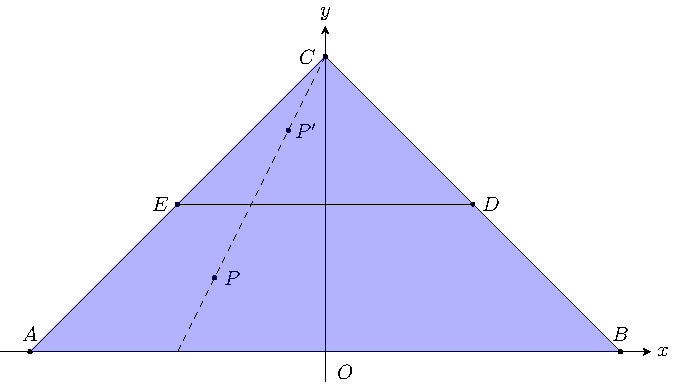
\includegraphics[scale=1]{images/fig_5.pdf}
                \end{center}
                \caption{Trapezoide $ABDE$.}
            \end{figure}
            y tomaremos a $E_2$ como el triángulo $ABC$. Definiremos una función $\cf{f}{E_1}{E_2}$ tal que el segmento $DE$ de la frontera de $E_1$ sea mapeada al vértice $C$ de $E_2$, pero en todos sus demás puntos sea una función biyectiva.

            Completaremos entonces la prueba diciendo que la topología cociente determinada por $f$ es la misma que la topología de $E_2$, esto para verificar que el espacio cociente de $E_1$ con su segmento es isomorfo a $E_2$, obteniendo así el resultado deseado.
            \item Definimos $f$ con la condición de que para todo $P=(x,y)\in E_1$, el punto $f(x,y)=P'=(x',y')\in E_2$ sea tal que esté en la recta que une a $P$ con $C=(0,1)$, dada de la siguiente manera:
            \begin{equation*}
                f(x,y)=\left(x\cdot\left(\frac{2y-1}{y-1}\right),2y \right)=(x',y'),\quad\forall (x,y)\in E_1
            \end{equation*}
            se verifica rápidamente que $g$ tiene como inversa en el conjunto $E_1$ menos el segmento $DE$ a la función $\cf{g}{E_2\setminus\left\{(0,1)\right\} }{E_1\setminus DE}$ dada por:
            \begin{equation*}
                g(x',y')=\left(x'\cdot\left(\frac{y'-2}{2y'-2} \right), \frac{1}{2}y'\right)=(x,y),\quad\forall (x',y')\in E_2\setminus\left\{(0,1) \right\} 
            \end{equation*}
            Es claro que $f$ es continua y que $g$ es la \textit{inversa} de $f$. Como $E_1$ es compacto y $E_2$ es Hausdorff, entonces $f$ es cerrada. Luego $E_2$ tiene la topología cociente inducida por $f$.
        \end{itemize}
    \end{proof}

    Estamos ahora listos para probar un lema fundamental. Sea $\cf{g}{I}{\mathbb{S}^1}$ (donde $\mathbb{S}^1$ denota la frontera de $\mathbb{D}^2$) la funcioń continua que da exactamente una vuelta alrededor del círculo, esto es
    \begin{equation*}
        g(0)=g(1)=d_0\in\mathbb{S}^1
    \end{equation*}
    esto es, que $g$ mapea el intervalo $(0,1)$ de forma homeomorfa en $B\setminus\left\{d_0 \right\}$.

    \begin{lema}
        Sea $X$ un espacio topológico. Una funcioń continua $\cf{f}{\mathbb{S}^1}{X}$ puede ser extendida a una función $\cf{F}{\mathbb{D}^2}{X}$ si y sólo si el bucle cerrado $\cf{f\circ g}{I}{X}$ es equivalente al bucle constante con punto base $f(d_0)$.
    \end{lema}

    \begin{proof}
        $\Rightarrow):$ Suponga que $\cf{f}{\mathbb{S}^1}{X}$ puede ser extendida a una función $\cf{F}{\mathbb{D}^2}{X}$. Considere el cuadrado unitario:
        \begin{equation*}
            S=\left\{ (x,y)\in\mathbb{R}^2\Big|0\leq x\leq 1\textup{ y }0\leq y\leq 1 \right\}
        \end{equation*}
        Definimos una función continua $\cf{h}{S}{\mathbb{S}^1}$ dada como sigue:
        \begin{equation*}
            \begin{split}
                h(x,0) &= g(x) \textup{ si } 0\leq x\leq 1\\
                h(x,1) &= h(0,y)=h(1,y)=d_0,\textup{ si }x\in I\textup{ o }y\in I \\
            \end{split}
        \end{equation*}
        Es claro que $h$ es continua. Por la proposición \ref{propB}, como $S\cong\mathbb{S}^1$, podemos extender $h$ a una función continua $\cf{H}{S}{\mathbb{S}^1}$. La función continua $\cf{F\circ H}{I\times I}{X}$ satisface que:
        \begin{equation*}
            \begin{split}
                F\circ H(x,0) &= F(h(x,0))\\
                &= F(g(x))\\
                &= f\circ g(x)\\
            \end{split}
        \end{equation*}
        y,
        \begin{equation*}
            \begin{split}
                F\circ H(x,1) &= F(h(x,1))\\
                &= F(d_0)\\
                &= f(d_0)\\
            \end{split}
        \end{equation*}
        para todo $x\in I$. Además,
        \begin{equation*}
            \begin{split}
                F\circ H(0,y) &= F(d_0) \\
                &= f(d_0)\\
            \end{split}
        \end{equation*}
        y,
        \begin{equation*}
            \begin{split}
                F\circ H(1,y) &= F(d_0) \\
                &= f(d_0)\\
            \end{split}
        \end{equation*}
        Por tanto, el bucle $f\circ g$ es equivalente al bucle constante con punto base $f(d_0)$.

        $\Leftarrow):$ Suponga que el bucle cerrado $f\circ g$ es equivalente al bucle constante con punto base $f(d_0)$. Entonces, existe una función continua $\cf{G}{I\times I}{X}$ tal que:
        \begin{equation*}
            \left\{
                \begin{split}
                    G(x,0) & = f\circ g(x)\\
                    G(x,1) & = G(0,y) = G(1,y) = f(d_0)\\
                \end{split}
            \right.,\quad\forall x\in I\textup{ y }\forall y\in I
        \end{equation*}
        notemos que de la segunda condición, $G$ mapea el borde superior y los dos bordes de $I\times I$ en un sólo punto, $f(d_0)$ en $X$, luego $G$ induce una función continua de este espacio cociente a $X$. Por la proposición anterior, este espacio cociente es un disco cerrado, digamos $\mathbb{D}^2$. Así que la función inducida $\cf{\widetilde{G}}{\mathbb{D}^2}{X}$ es tal que la frontera de %TODO
        \begin{equation*}
            \begin{split}
                \widetilde{G}(x,y)=
            \end{split}
        \end{equation*}
    \end{proof}

    Aplicando el lema anterior, es conveniente usar el siguiente abuso de notación, diremos que la función $\cf{f}{\mathbb{S}^1}{X}$ \textit{representa} la clase de equivalencia del bucle $f\circ g$.

    \begin{theor}
        Sean $X$ y $Y$ espacios topológicos, $\cf{\varphi_0,\varphi_1}{X}{Y}$ funciones continuas homotópicas y sea $\cf{\varphi}{X\times I}{Y}$ la homotopía entre ambas funciones. Sea $x_0\in X$ y considere los homomorfismos inducidos por $\varphi_0$ y $\varphi_1$:
        \begin{equation*}
            \left\{
            \begin{split}
                &\cf{{\varphi_0}_*}{\pi(X,x_0)}{\pi(Y,\varphi_0(x_0))}\\
                &\cf{{\varphi_1}_ }{\pi(X,x_0)}{\pi(Y,\varphi_1(x_0))}\\
            \end{split}
            \right.
        \end{equation*}
        Sea $[\gamma]$ la clase de equivalencia del camino $\cf{\gamma}{I}{Y}$, dado por $t\mapsto\varphi_0(x_0,t)$. Considere el isomorfismo inducido $\cf{u}{\pi(Y,\varphi_0(x_0))}{\pi(Y,\varphi_1(x_0))}$ dado por:
        \begin{equation*}
            u([f])=[\gamma]^{-1}\cdot[f]\cdot[\gamma],\quad\forall [f]\in\pi(Y,\varphi_0(x_0))
        \end{equation*}
        Entonces, el diagrama

        \begin{minipage}{\textwidth}
            \begin{center}
                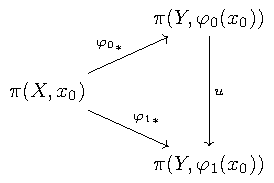
\includegraphics[scale=1.5]{images/fig_4.pdf}\\
                Figura 2.3. Conmutatividad de $\pi(X,x_0)$, $\pi(Y,\varphi_0(x_0))$ y $\pi(Y,\varphi_1(x_0))$.
            \end{center}
        \end{minipage}

        es conmutativo.
    \end{theor}

    \begin{proof}
        %TODO
    \end{proof}

    Note que este teorema es una generalización de un teorema anterior. 

    \begin{mydef}
        Dos espacios topológicos $X$ y $Y$ tienen el \textbf{mismo tipo de homotopía} si existen funciones continuas, llamadas \textbf{equivalencias de homotopía}, $\cf{f}{X}{Y}$ y $\cf{g}{Y}{X}$ tales que:
        \begin{equation*}
            g\circ f\simeq\bbm{1}_X\quad\textup{y}\quad f\circ g\simeq\bbm{1}_Y
        \end{equation*}
    \end{mydef}

    Se sigue de forma inmediata que dos espacios homeomorfos tienen el mismo tipo de homotopía, pero el converso no es cierto (en general).

    \begin{theor}
        Si $\cf{f}{X}{Y}$ es una equivalencia de homotopía, entonces $\cf{f_*}{\pi(X,x)}{\pi(Y,f(x))}$ es un isomorfismo, para todo $x\in X$.
    \end{theor}

    \begin{proof}
        %TODO
    \end{proof}

    Este teorema será usado como mira para determinar los grupos fundamentales de ciertos espacios, y como un método de probar que ciertos espacios no tienen el mismo tipo de homotopía (y en consecuencia, no son homeomorfos).

    \newpage

    \section{Ejercicios}

    \begin{excer}
        Pruebe que un espacio conexo y localmente arco-conexo es arco conexo.
    \end{excer}

    \begin{proof}
        
    \end{proof}

    \begin{excer}
        ¿Bajo qué condiciones dos clases de caminos que unen a $x$ y $y$ se tendrá el mismo isomorfismo entre de $\pi(X,x)$ y $\pi(X,y)$?
    \end{excer}

    \begin{sol}
        
    \end{sol}

    \begin{excer}
        Sea $X$ un espacio arco conexo. ¿Bajo qué condiciones es la siguiente proposición válida? Para cualesquiera dos puntos $x,y\in X$ todas las clases de caminos de $x$ a $y$ dan el mismo isomorfismo entre $\pi(X,x)$ y $\pi(X,y)$. 
    \end{excer}

    \begin{sol}
        
    \end{sol}

    \begin{excer}
        Sean $\cf{f,g}{I}{X}$ dos caminos con punto inicial $x_0$ y final $x_1$. Pruebe que $f\sim g$ si y sólo si $f\cdot\overline{g}$ es equivalente al camino constante en $x_0$ (recordando que $\overline{g}$ es el camino que invierte la forma de recorrer a $g$).
    \end{excer}

    \begin{proof}
        
    \end{proof}

    \begin{excer}
        Sean $\cf{\varphi}{X}{Y}$ una función continua y $[f]$ una clase de camino en $X$ que va de $x_0$ a $x_1$. Pruebe que el siguiente diagrama es conmutativo:
        \begin{equation*}
            \begin{array}{rcccl}
              & \pi(X,x_0) & \overset{\varphi_*}{\longrightarrow} & \pi(Y,\varphi(x_0)) & \\
              u & \downarrow & & \downarrow & v \\
               & \pi(X,x_1) & \overset{\varphi_*}{\longrightarrow} & \pi(Y,\varphi(x_1)) & \\
            \end{array}
        \end{equation*}
        donde $u$ es el homomorfismo definido como: $u([g])=[f]^{-1}\cdot[g]\cdot[f]$ y $v$ se define de forma similar usando $\varphi_*([f])$ en lugar de $[f]$. ¿Qué sucede si $\varphi(x_0)=\varphi(x_1)$?
    \end{excer}

    \begin{proof}
        
    \end{proof}

    \begin{excer}
        Construya una deformación de retracción de $\mathbb{R}^n$ en $S^{ n-1}$.
    \end{excer}

    \begin{sol}
        
    \end{sol}

    \begin{excer}
        Pruebe que un repliegue de un espacio Hausdorff debe ser un conjunto cerrado.
    \end{excer}

    \begin{proof}
        
    \end{proof}

    \begin{excer}
        Pruebe que si $A$ es un repliegue de $X$ y $\cf{r}{X}{A}$ es una retracción, $\cf{i}{A}{X}$ es el mapeo inclusión, $a\in A$ es arbitrario fijo y $i_*(\pi(A,a))$ es un subgrupo normal de $\pi(X,a)$, entonces $\pi(X,a)$ es el producto directo de los subgrupos
        \begin{equation*}
            i_*(\pi(A,a))\quad\textup{y}\quad \ker(r_*)
        \end{equation*}
    \end{excer}

    \begin{proof}
        
    \end{proof}

    \begin{excer}
        Sea $A$ un subespacio de $X$, y sea $Y$ un espacio topológico no vacío. Pruebe que $A\times Y$ es un repliegue de $X\times Y$ si y sólo si $A$e s una repliegue de $X$.
    \end{excer}

    \begin{proof}
        
    \end{proof}

    \begin{excer}
        Pruebe que la relación \textbf{ser repliegue de} es transitiva, esto es, si $A$ es un repliegue de $B$ y $B$ es un repliegue de $C$, entonces $A$ es un repliegue de $C$.
    \end{excer}

    \begin{proof}
        
    \end{proof}

    \begin{excer}
        Sea $x_0\in\mathbb{R}^2$. Encuentre un círculo $C\subseteq\mathbb{R}^2$ tal que es un repliegue de deformación de $\mathbb{R}^2-\left\{x_0\right\}$. Generalice este resultado a $n$-dimensiones.
    \end{excer}

    \begin{proof}
        
    \end{proof}

    \begin{excer}
        Sea $\mathbb{T}$ un toro y considere $X=\mathbb{T}-\left\{x\right\}$, con $x\in\mathbb{T}$. Encuentre un subconjunto de $X$ que sea homeomorfo a la figura \textit{8} (esto es, la unión de dos círculos con un punto en común) y que es una retracción de deformación de $X$.
    \end{excer}

    \begin{proof}
        
    \end{proof}

    \begin{excer}
        Sean $x,y\in X$ dos puntos distintos en un espacio simplemente conexo $X$. Pruebe que existe una \textit{única} clase de caminos en $X$ que une al punto inicial $x$ con el punto final $y$.
    \end{excer}

    \begin{proof}
        
    \end{proof}

    \begin{excer}
        Sea $X$ un espacio topológico y, para número natural $n\in\mathbb{N}$ sea $X_n$ un subespacio arco-conexo que contiene como punto base $x_0\in X$. Asuma que los subespacios están enacajados, esto es
        \begin{equation*}
            X_n\subseteq X_{ n+1},\quad\forall n\in\mathbb{N}
        \end{equation*}
        y que
        \begin{equation*}
            X=\bigcup_{ n=1}^{\infty}X_n
        \end{equation*}
        además, para cada subconjunto compacto $A\subseteq X$ existe $m\in\mathbb{N}$ tal que $A\subseteq X_m$. Sean
        \begin{equation*}
            \cf{i_n}{\pi(X_n,x_0)}{\pi(X,x_0)}\quad\textup{y}\quad \cf{j_{ mn}}{\pi(X_m,x_0)}{\pi(X_n,x_0)}
        \end{equation*}
        los homomorfismos inducidos por las funciones inclusión, para todo $n\in\mathbb{N}$ y $m\in\mathbb{N}$ tal que $m<n$. Pruebe lo siguiente:
        \begin{enumerate}
            \item Para cada $[f]\in\pi(X,x_0)$ existe un natural $n\in\mathbb{N}$ y un elemento $[g]\in\pi(X_n,x_0)$ tal que $i_n([g])=[f]$.
            \item Si $[f]\in\pi(X_m,x_0)$ e $i_m([f])=1$, entonces existe un entero $n\geq m$ tal que $j_{ mn}([f])=1$.
            \item Si los homomorfismos $j_{ n,n+1}$ son monomorfismos para todo $n\in\mathbb{N}$, pruebe que cada $i_n$ es un monomorfismo y que $\pi(X,x_0)$ es la unión de los subgrupos $i_n(\pi(X_n,x_0))$.
        \end{enumerate}
    \end{excer}

    \begin{proof}
        
    \end{proof}

    %TODO Ejercicios de la sección 5

    \begin{excer}
        Sea $\left\{U_i \right\}_{ i\in I}$ una cubierta abierta del espacio $X$ con las siguientes propiedades:
        \renewcommand{\theenumi}{\alph{enumi}}
        \begin{enumerate}
            \item Existe un punto $x_0\in X$ tal que $x_0\in U_i$ para todo $i\in I$.
            \item Cada $U_i$ es simplemente conexo.
            \item Si $i\neq j$ con $i,j\in I$, entonces $U_i\cap U_j$ es arco-conexo. 
        \end{enumerate}
        pruebe que $X$ es simplemente conexo.
        
        \textit{Sugerencia}: Para probar que cualquier bucle $\cf{f}{I}{X}$ con punto base $x_0$ es trivial, considere la cubierta abierta $\left\{f^{-1}(U_i) \right\}_{ i\in I}$ del espacio métrico compacto $I$ y haga uso del número de Lebesgue de esta cubierta.
    \end{excer}

    \begin{proof}
        
    \end{proof}

    \begin{obs}
        En el ejercicio anterior existen dos casos importantes:
        \begin{enumerate}
            \item $X$ es cubierto por dos conjuntos abiertos.
            \item Los conjuntos $U_i$ están linealmente ordenados por la inclusión.
        \end{enumerate}
    \end{obs}

    \begin{excer}
        Reescriba el ejercicio anterior con las hipótesis de la observación anterior y explique qué está sucediendo.
    \end{excer}

    \begin{proof}
        
    \end{proof}

    \begin{excer}
        Use el resultado del ejercicio anterior (la parte $a$)) para probar que $\mathbb{S}^2$ es simplemente conexo. Generalice este resultado para probar que $\mathbb{S}^n$ es simplemente conexo.
    \end{excer}

    \begin{proof}
        
    \end{proof}

    \begin{excer}
        Pruebe que $\mathbb{R}^2$ y $\mathbb{R}^n$ no son homeomorfos.

        \textit{Sugerencia}. Considere el complemento de un punto en $\mathbb{R}^2$ o $\mathbb{R}^n$.
    \end{excer}

    \begin{proof}
        
    \end{proof}

    \begin{excer}
        Pruebe que cualquier homeomorfismo del disco cerrado $\bbm{D}^2$ en sí mismo mapea a $\mathbb{S}^1$ en sí mismo y a $\bbm{U}^2$ en sí mismo, donde
        \begin{equation*}
            \bbm{U}^2=\left\{(x,y)\in\bbm{R}^2\Big|x^2+y^2<1 \right\}
        \end{equation*}
    \end{excer}

    \begin{proof}
        
    \end{proof}
    
    \begin{excer}
        Describa el grupo fundamental del toro.

        \textit{Sugerencia.} Recuerde que $\bbm{T}=\bbm{S}^1\times\bbm{S}^1$.
    \end{excer}

    \begin{proof}
        
    \end{proof}

    \begin{excer}
        Pruebe que el subconjunto $\bbm{S}^1\times\left\{x_0 \right\}$ es una retracción de $\bbm{S}^1\times\bbm{S}^1$, pero que no es un repliegue de deformación, para cualquier $x_0\in\bbm{S}^1$.
    \end{excer}

    \begin{proof}
        
    \end{proof}

    \begin{excer}
        Sea $\cf{i}{X}{X\times Y}$ y $\cf{j}{Y}{X\times Y}$ las funciones definidas por:
        \begin{equation*}
            i(x)=(x,y_0)\quad\textup{y}\quad j(y)=(x_0,y)
        \end{equation*}
        para todo $x\in X$ y para todo $y\in Y$, siendo $x_0\in X$ y $y_0\in Y$. Pruebe que la función $\cf{\Gamma}{\pi(X,x_0)\times\pi(Y,y_0)}{\pi(X\times Y,(x_0,y_0))}$ dado por:
        \begin{equation*}
            \Gamma([f],[g])=(i_*([f]))\cdot(j_*([g]))
        \end{equation*}
        para todo $[f],[g]\in\pi(X,x_0)\times\pi(Y,y_0)$, es un isomorfismo de grupos.

        Más aún, deduzca que
        \begin{equation*}
            (i_*([f]))\cdot(j_*([g]))=(j_*([g]))\cdot(i_*([f]))
        \end{equation*}
        para todo $[f]\in\pi(X,x_0)$ y para todo $[g]\in\pi(Y,y_0)$.

        \textit{Sugerencia.} Pruebe que es el isomorfismo inverso del teorema que caracteriza el grupo fundamental del producto de dos espacios topológicos. 
    \end{excer}

    \begin{proof}
        
    \end{proof}

    \begin{excer}
        Sea $G$ un espacio topológico, $\cf{\mu}{G\times G}{G}$ una función y $e\in G$ tal que
        \begin{equation*}
            \mu(e,g)=\mu(g,e)=g,\quad\forall g\in G
        \end{equation*}
        Considere las funciones $\cf{i}{G}{G\times G}$ y $\cf{j}{G}{G\times G}$ dadas por:
        \begin{equation*}
            i(x)=(x,e)\quad\textup{y}\quad j(y)=(e,y)
        \end{equation*}
        para todo $x,y\in G$. Pruebe que para cualesquier par de elementos $[f],[g]\in\pi(G,e)$ se cumple que:
        \begin{equation*}
            \mu_*\left(i_*([f]),j_*([g]) \right)=[f]\cdot[g]
        \end{equation*}
        Deduzca que $\pi(G,e)$ es un grupo abeliano.
    \end{excer}

    \begin{proof}
        
    \end{proof}

    \begin{excer}
        Sean $G,e$ y $\mu$ como en el ejercicio anterior. Suponga que existe una función $\cf{c}{G}{G}$ tal que:
        \begin{equation*}
            \mu(x,c(x))=\mu(c(x),x)=e,\quad\forall x\in G
        \end{equation*}
        Pruebe que para todo $[f]\in\pi(G,e)$ se cumple:
        \begin{equation*}
            c_*([f])=[f]^{-1}
        \end{equation*}
    \end{excer}

    \begin{proof}
        
    \end{proof}
    
    \begin{obs}
        En particular, en los ejercicios anteriores podemos considerar un grupo topológico $(G,\cdot,\tau)$.
    \end{obs}

    \begin{excer}
        Pruebe que si $A$ es un repliegue de deformación de $X$, entonces el mapeo inclusión $\cf{i}{A}{X}$ es una equivalencia de homtopía.
    \end{excer}

    \begin{proof}
        
    \end{proof}

    \begin{excer}
        Suponga que $G,e,\mu$ satisfacen las condiciones del Ejercicio 2.10.23. Use el Lema 2.9.1 para probar directamente que para cualquier par de elementos $[f],[g]\in\pi(G,e)$ se cumple:
        \begin{equation*}
            [f]\cdot[g]\cdot[f]^{-1}\cdot[g]^{-1}=\bbm{1}
        \end{equation*}
        donde $\bbm{1}$ es la unidad de $\pi(G,e)$. Deduzca que $\pi(G,e)$ es abeliano.
    \end{excer}

    \begin{proof}
        
    \end{proof}

\end{document}